\documentclass[runningheads]{llncs}
\usepackage{amsmath}
\usepackage{amssymb}
\usepackage{graphicx}
\usepackage{cite}
\usepackage{array}
\usepackage{xltabular}
\usepackage{booktabs}
\usepackage{float}
\usepackage{placeins}
\usepackage{hyperref}
\usepackage{tikz}
\usetikzlibrary{positioning, fit, arrows.meta, backgrounds}
\usepackage[ruled,vlined,linesnumbered]{algorithm2e}
\SetKwInput{KwInput}{Input}
\SetKwInput{KwOutput}{Output}
\SetKwProg{Fn}{Function}{:}{}
\SetKwProg{Proc}{Procedure}{:}{}

\title{A Comparative Analysis of Energy Efficiency Across Large Language Models}
\titlerunning{A Comparative Analysis of Energy Efficiency Across LLMs}

\author{Fatin Israq Talha \and
Mehrab Sadekin Borno \and
Md Rakib Hasan Rabbi \and
Muhmmad Ahamadul Hasan Prianto}

% Suppress author running head ("Authors Suppressed Due to Excessive Length")
\authorrunning{ }
% When you want to display authors in the running head later, uncomment below:
% \authorrunning{F. I. Talha et al.}


\institute{Department of Computer Science and Engineering,\\
United International University, Dhaka, Bangladesh}

\begin{document}

\maketitle

\begin{abstract}
The rapid adoption of large language models has led to a common but energy-inefficient practice: routing all user prompts, regardless of complexity, through the same large-scale model. This uniform approach incurs substantial and often unnecessary energy costs, as many prompts do not require the full capacity of a large model to be answered accurately. In this work, we first conduct an empirical study measuring the energy consumption and output quality of multiple open-source language models across varying sizes and quantization levels, using real-time GPU power measurements. Building on these measurements, we propose a lightweight prompt-complexity router that dynamically selects the smallest capable model for a given input, reserving larger models only for prompts that genuinely require them. We evaluate our system in terms of total energy consumption, response quality, and latency, comparing it against a baseline that always uses a single large model. Our results demonstrate that adaptive model routing can substantially reduce energy consumption with minimal degradation in answer quality, offering a practical and generalizable strategy for building more sustainable AI-serving systems.

\keywords{Large Language Models \and Energy Efficiency \and Green Computing \and Model Quantization \and Model Routing \and Sustainable AI}
\end{abstract}

\section{Introduction}
\label{sec:introduction}
 
The past several years have seen an unprecedented surge in Large Language Model adoption across consumer, enterprise, and scientific applications. Models such as GPT, Llama, and Mistral now process billions of daily inference requests spanning simple lookups to multi-step reasoning. However, this deployment demands massive computational and energy resources, raising pressing sustainability concerns within the Green AI community~\cite{strubell2019energy, schwartz2020greenai}.
 
Much of this energy consumption stems from a pervasive architectural inefficiency: routing every query to the same large model regardless of complexity. A trivial classification query and an intricate mathematical proof are allocated identical capacity, even though smaller, quantized models can resolve simpler tasks at a fraction of the energy cost. At scale, this uniform, ``one-size-fits-all'' serving strategy incurs substantial and unnecessary environmental footprints~\cite{strubell2019energy}.

Prior research addresses this challenge through three largely disconnected paradigms: (i)~\emph{hardware measurement}, profiling real-world GPU power draw during inference to establish empirical baselines~\cite{samsi2023words, fernandez2025energy, wilkins2024hybrid, ji2025systematic, niu2026tokenpowerbench}; (ii)~\emph{model compression}, applying post-training quantization to reduce memory and compute overheads~\cite{frantar2022gptq, li2023thirsty, xiao2023smoothquant, dettmers2022llmint8}; and (iii)~\emph{model routing}, dynamically escalating queries across diverse model tiers~\cite{chen2023frugalgpt, ong2024routellm, ding2024hybridllm, khan2025optimizing}. Crucially, these domains remain unintegrated: measurement benchmarks rarely inform serving-time decisions, quantization is seldom treated as a dynamic routing dimension, and routing frameworks optimize primarily for monetary cost or latency rather than measured hardware energy draw.
 
Consequently, existing literature lacks a framework that simultaneously (i) directly measures inference energy via real-time GPU power sampling, (ii) incorporates quantization level as a primary routing parameter, and (iii) makes per-prompt routing decisions based on query complexity at serving time. Bridging this gap is the central motivation of our work.
 
To this end, we make the following contributions:
 
\begin{itemize}
    \item We conducted an empirical energy-profiling study across multiple open-source LLMs spanning different parameter scales and quantization levels, capturing real-time GPU power draw via NVML on consumer-grade hardware.
    \item Using these measurements, we designed and implemented a lightweight, prompt-complexity-aware router that dynamically dispatches each query to the smallest capable quantized model tier, reserving larger models for complex reasoning tasks.
    \item We evaluated the resulting adaptive-routing framework against a static single-large-model baseline across total energy, quality retention, and end-to-end latency using a multi-tier benchmark workload.
\end{itemize}
 
Our experimental results demonstrate that adaptive, complexity-aware routing substantially reduces inference energy consumption with minimal quality degradation relative to a static large-model baseline, offering a practical and hardware-grounded strategy for sustainable LLM serving.

The remainder of this paper is organized as follows. Section~\ref{sec:related-works} reviews related literature across energy profiling, model compression, and inference routing strategies, followed by a comparative gap analysis. Section~\ref{sec:methodology} details the proposed methodology, outlining the system architecture, tiered quantized model pool, lightweight prompt-complexity routing pipeline, and hardware-level energy measurement setup. Section~\ref{sec:results} presents the empirical evaluation and cross-platform results across two GPU microarchitectures, analyzing dynamic energy savings, task quality retention, microarchitectural scaling behavior, and serving latency overheads, concluding with core architectural takeaways.

\section{Related Works}
\label{sec:related-works}

\subsection{Literature Review}

The growing energy footprint of large language model (LLM) inference has motivated a substantial body of work that can be organized into four broad, interconnected strands: (i) empirical measurement of LLM inference energy, (ii) quantization as a means of reducing the energy-accuracy trade-off, (iii) model routing and cascading strategies that avoid invoking large models unnecessarily, and (iv) foundational work establishing the carbon and environmental footprint of deep learning and motivating the broader Green AI agenda.

A first line of work focuses on directly profiling the energy consumed during LLM inference under real hardware conditions. Samsi et al.~\cite{samsi2023words} benchmark the energy costs of several open-source LLMs on GPU infrastructure, establishing baseline power and latency figures that later routing and quantization studies build upon. Fernandez et al.~\cite{fernandez2025energy} extend this measurement effort by explicitly considering efficiency optimizations, framing energy consumption as a first-class metric alongside accuracy and latency. Complementing these single-node measurement studies, Wilkins et al.~\cite{wilkins2024hybrid} show that heterogeneous GPU clusters can be scheduled to lower the aggregate energy consumption of inference workloads, suggesting that energy savings can be achieved not only at the model level but also at the infrastructure-scheduling level. Ji and Jiang~\cite{ji2025systematic} provide a systematic review of electricity demand associated with LLMs, consolidating evaluation methodologies and open challenges across the field. Most recently, Niu et al.~\cite{niu2026tokenpowerbench} introduce TokenPowerBench, a benchmark that captures GPU-, node-, and system-level power draw and attributes energy separately to the prefill and decode phases of inference, offering fine-grained evidence that informs the design of measurement pipelines such as the one used in this project.

A second strand investigates quantization as a direct lever for reducing the energy cost of inference while attempting to preserve output quality. Frantar et al.~\cite{frantar2022gptq} introduce GPTQ, a post-training quantization method that compresses model weights with minimal accuracy loss, and Lin et al.~\cite{lin2024awq} propose AWQ, which protects a small subset of salient weights to further improve the accuracy-compression trade-off. Xiao et al.~\cite{xiao2023smoothquant} address the difficulty of quantizing activations by smoothing outlier values prior to quantization, and Dettmers et al.~\cite{dettmers2022llmint8} demonstrate that 8-bit matrix multiplication can match full-precision performance at large model scale. Collectively, this strand establishes that quantization level is a controllable variable that trades a measurable amount of accuracy for a measurable amount of energy savings -- precisely the trade-off this project seeks to characterize empirically.

A third strand, closely aligned with the routing component of this project, explores directing individual prompts to different models based on estimated complexity, rather than applying quantization uniformly. Chen et al.~\cite{chen2023frugalgpt} propose FrugalGPT, a cascading strategy that queries progressively larger LLMs only when earlier, cheaper models are deemed insufficiently confident, substantially reducing cost while retaining accuracy. Ong et al.~\cite{ong2024routellm} learn a routing function from human-preference data to decide, per query, whether a smaller or larger model should respond. Ding et al.~\cite{ding2024hybridllm} formalize a similar problem as cost-efficient, quality-aware query routing between a small and a large model. Khan et al.~\cite{khan2025optimizing} present a case study connecting routing-style optimizations to energy-efficiency metrics specifically, rather than cost alone. While these works demonstrate that routing can reduce inference cost or latency, comparatively few directly measure the resulting energy savings using real-time hardware power measurements, which is a gap this project's proposed router is designed to address.

Finally, a foundational strand of work established the environmental case for energy-aware AI system design in the first place. Strubell et al.~\cite{strubell2019energy} were among the first to quantify the carbon emissions of training large NLP models, prompting widespread attention to the sustainability of deep learning research. Schwartz et al.~\cite{schwartz2020greenai} formalize the notion of ``Green AI,'' arguing for efficiency as an explicit research objective alongside accuracy. Li et al.~\cite{li2023thirsty} draw attention to the often-overlooked water footprint of AI model training and serving. Luccioni et al.~\cite{luccioni2023bloom} provide a detailed carbon-footprint case study of the 176B-parameter BLOOM model, illustrating the scale of emissions associated with large-model deployment. Together, these works motivate the broader problem this project addresses: reducing the operational energy footprint of LLM inference through model-level and system-level design choices.

\subsection{Gap Analysis}

Table~\ref{tab:gap-analysis} summarizes the reviewed literature according to problem definition, contribution, methodology, and the specific gap that motivates the present work. Across the reviewed studies, three recurring gaps emerge. First, energy-measurement studies~\cite{samsi2023words,fernandez2025energy,wilkins2024hybrid,ji2025systematic,niu2026tokenpowerbench} establish sound measurement methodology but rarely combine those measurements with an actionable serving-time decision mechanism. Second, quantization studies~\cite{frantar2022gptq,lin2024awq,xiao2023smoothquant,dettmers2022llmint8} characterize the energy-accuracy trade-off of compressing a single model but do not consider dynamically choosing among multiple models of different sizes per prompt. Third, routing and cascading studies~\cite{chen2023frugalgpt,ong2024routellm,ding2024hybridllm,khan2025optimizing} optimize primarily for monetary cost or latency, with energy treated as, at best, a secondary or estimated metric rather than one measured directly from GPU power draw. This project is positioned to close these gaps by combining direct, real-time GPU energy measurement (as in the first strand) with a prompt-complexity router (as in the third strand) that additionally accounts for quantization level (as in the second strand) when selecting a model, and by evaluating the resulting system explicitly on measured energy consumption rather than proxy cost metrics.

As summarized above, no reviewed work simultaneously (1) measures LLM inference energy directly via real-time GPU power draw, (2) incorporates model quantization level as a routing variable, and (3) makes a per-prompt, complexity-aware model-selection decision at serving time. This combined gap is the primary motivation for the energy-aware prompt-complexity router proposed in this work.

\begingroup
\footnotesize
\setlength{\tabcolsep}{3pt}
\renewcommand{\arraystretch}{1.15}

\begin{xltabular}{\textwidth}{|>{\raggedright\arraybackslash}p{1.2cm}|>{\raggedright\arraybackslash}X|>{\raggedright\arraybackslash}X|>{\raggedright\arraybackslash}X|>{\raggedright\arraybackslash}X|}
\caption{Gap analysis of the papers most closely related to this project.}
\label{tab:gap-analysis} \\
\hline
\textbf{Ref.} & \textbf{Problem Definition} & \textbf{Contribution} & \textbf{Methodology} & \textbf{Gap Found} \\
\hline
\endfirsthead

\caption[]{Gap analysis of the papers most closely related to this project. (\textit{Continued})} \\
\hline
\textbf{Ref.} & \textbf{Problem Definition} & \textbf{Contribution} & \textbf{Methodology} & \textbf{Gap Found} \\
\hline
\endhead

\hline
\multicolumn{5}{|r|}{\footnotesize\textit{Continued on next page}} \\
\hline
\endfoot

\hline
\endlastfoot

\cite{samsi2023words} &
Lack of standard LLM inference energy benchmarks. &
Benchmarked GPU energy costs across open-source LLMs. &
Measured GPU power draw over fixed prompt sets. &
Static profiling only; lacks runtime model selection or routing. \\
\hline

\cite{niu2026tokenpowerbench} &
Lack of phase-specific power attribution in inference profiling. &
TokenPowerBench: phase-aware power measurement (prefill vs.\ decode). &
Profiles varied LLMs across contexts, batches, and quantizations (J/tok). &
Offline profiling framework; no per-prompt model or quantization routing. \\
\hline

\cite{chen2023frugalgpt} &
Uniform large-model serving incurs excessive API/monetary costs. &
FrugalGPT: cascading strategy querying cheaper LLMs first. &
Confidence-based cascading across commercial LLM APIs. &
Optimized for monetary cost and accuracy; ignores hardware energy draw. \\
\hline

\cite{ong2024routellm} &
Need automated query routing between small and large LLMs. &
RouteLLM: preference-trained router for small vs.\ large models. &
Trained classifier on human preferences for query dispatch. &
Tuned for response quality and cost; ignores physical energy consumption. \\
\hline

\cite{khan2025optimizing} &
Disconnect between LLM optimization techniques and real energy impact. &
Case study linking various optimizations to energy outcomes. &
Evaluated existing optimizations against energy and runtime metrics. &
Retrospective analysis; lacks a live complexity router for energy reduction. \\
\hline

\end{xltabular}

\endgroup

\FloatBarrier
\vspace{1.5em}

\section{Methodology}
\label{sec:methodology}

This section details the experimental methodology developed to systematically investigate and leverage the energy-quality trade-offs inherent in large language model inference. The proposed framework integrates three core components: an adaptive serving architecture backed by a tiered, quantized model pool; a lightweight, low-overhead prompt-complexity routing mechanism; and a multi-platform hardware testbed coupled with real-time GPU power instrumentation and multi-dimensional evaluation metrics.

\subsection{System Architecture and Quantized Model Tiers}
\label{subsec:system-architecture}

The overarching system architecture, illustrated in Figure~\ref{fig:system-architecture}, is designed to eliminate the computational and energetic waste of uniform model serving by dynamically matching query complexity to model capacity. When an incoming user prompt arrives, it is first intercepted at the host level where syntactic and semantic features are extracted to determine task difficulty. The request is then dispatched to the smallest capable model tier residing in GPU memory. During subsequent autoregressive token generation, an isolated background profiler records real-time power draw to compute precise energy consumption, after which the generated response, latency profile, and power statistics are aggregated for evaluation.

\begin{figure}[htbp]
\centering
\resizebox{\textwidth}{!}{%
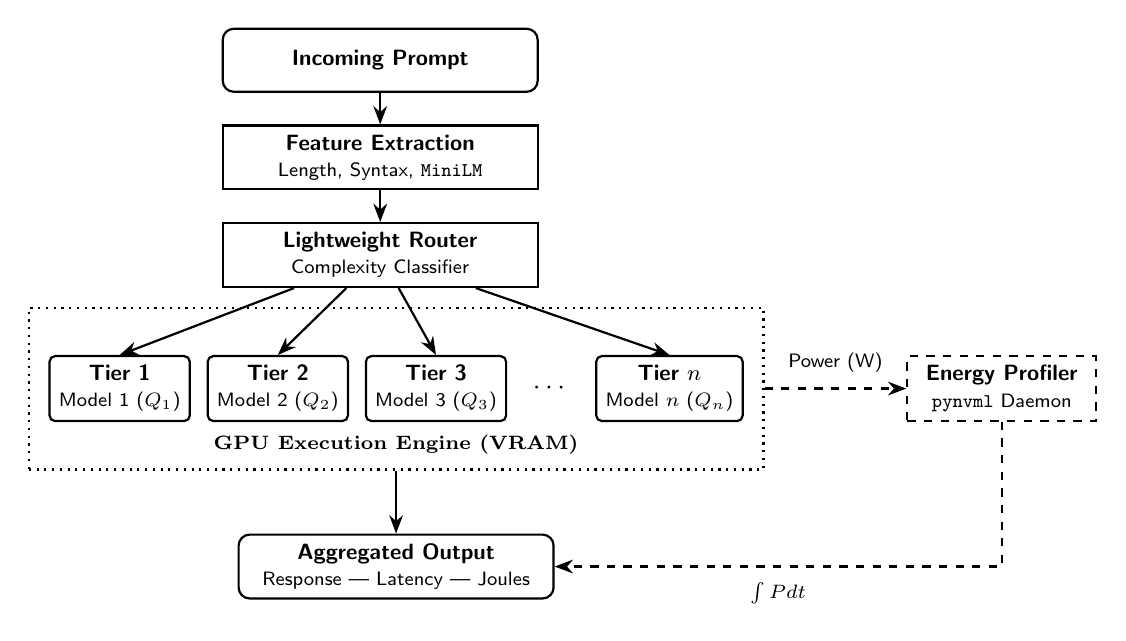
\begin{tikzpicture}[
    font=\sffamily\footnotesize,
    >=Stealth,
    main_box/.style={draw, thick, minimum width=4.0cm, minimum height=0.8cm, align=center, fill=white},
    tier_box/.style={draw, thick, minimum width=1.6cm, minimum height=0.8cm, align=center, fill=white, rounded corners=2pt},
    profiler_box/.style={draw, thick, dashed, minimum width=2.4cm, minimum height=0.8cm, align=center, fill=white},
    arrow/.style={->, thick},
    dash_arrow/.style={->, thick, dashed}
]

% Top-down Nodes
\node[main_box, rounded corners=4pt] (prompt) {\textbf{Incoming Prompt}};
\node[main_box, below=0.4cm of prompt] (fe) {\textbf{Feature Extraction}\\ \scriptsize Length, Syntax, \texttt{MiniLM}};
\node[main_box, below=0.4cm of fe] (router) {\textbf{Lightweight Router}\\ \scriptsize Complexity Classifier};

% Model Tiers (Generic Tier 1 through Tier n)
\node[tier_box, below=0.85cm of router, xshift=-1.3cm] (tier2) {\textbf{Tier 2}\\ \scriptsize Model 2 ($Q_2$)};
\node[tier_box, left=0.2cm of tier2] (tier1) {\textbf{Tier 1}\\ \scriptsize Model 1 ($Q_1$)};
\node[tier_box, right=0.2cm of tier2] (tier3) {\textbf{Tier 3}\\ \scriptsize Model 3 ($Q_3$)};
\node[right=0.2cm of tier3, minimum width=0.6cm, font=\bfseries\normalsize] (dots) {$\cdots$};
\node[tier_box, right=0.2cm of dots] (tiern) {\textbf{Tier $n$}\\ \scriptsize Model $n$ ($Q_n$)};

% Bounding box representing the GPU
\node[draw, thick, dotted, inner xsep=0.25cm, inner ysep=0.6cm, fit=(tier1)(tier2)(tier3)(dots)(tiern)] (gpu) {};
\node[above=0.08cm of gpu.south, font=\bfseries\scriptsize] {GPU Execution Engine (VRAM)};

% Profiler Daemon
\node[profiler_box, right=1.8cm of gpu] (profiler) {\textbf{Energy Profiler}\\ \scriptsize \texttt{pynvml} Daemon};

% Final Output
\node[main_box, rounded corners=4pt, below=0.8cm of gpu] (output) {\textbf{Aggregated Output}\\ \scriptsize Response | Latency | Joules};

% Routing connections
\draw[arrow] (prompt) -- (fe);
\draw[arrow] (fe) -- (router);
\draw[arrow] (router) -- (tier1.north);
\draw[arrow] (router) -- (tier2.north);
\draw[arrow] (router) -- (tier3.north);
\draw[arrow] (router) -- (tiern.north);
\draw[arrow] (gpu.south) -- (output.north);

% Profiling connections
\draw[dash_arrow] (gpu.east) -- (profiler.west) node[midway, above=2pt] {\scriptsize Power (W)};
\draw[dash_arrow] (profiler.south) |- (output.east) node[near end, below=2pt] {\scriptsize $\int P dt$};

\end{tikzpicture}%
}
\caption{Generic system architecture pipeline demonstrating the adaptive routing mechanism across $n$ candidate model tiers and real-time energy profiling.}
\label{fig:system-architecture}
\end{figure}

To replicate practical, cost-effective deployments on consumer workstations and edge servers, the candidate model pool is structured to operate under a strict 8\,GB VRAM budget. To evaluate and determine the optimal architecture for each tier, we deploy a comparative matrix of two candidate models per tier across three distinct operational tiers (six models total), pairing open-weight architectures with tailored post-training quantization schemes via the GGUF container format:

\emph{Tier 1 (Lightweight / Low Complexity):} Designed for minimal active power draw and rapid execution, Tier~1 deploys compact parameter architectures: \texttt{Llama-3.2-1B-Instruct} (1.24B parameters, \texttt{Q8\_0}, $\sim 1.3$\,GB VRAM) and \texttt{Qwen-2.5-1.5B-Instruct} (1.54B parameters, \texttt{Q4\_K\_M}, $\sim 1.0$\,GB VRAM). Retaining high quantization precision preserves token representation and semantic fidelity on low-complexity tasks---such as binary sentiment classification (SST-2) and short factual extraction (SQuAD v2.0)---while executing with minimal computational arithmetic and abbreviated GPU active states.

\emph{Tier 2 (Intermediate / Medium Complexity):} Serving as the mid-tier workhorse, Tier~2 incorporates mid-sized models: \texttt{Llama-3.2-3B-Instruct} (3.21B parameters, \texttt{Q4\_K\_M}, $\sim 2.0$\,GB VRAM) and \texttt{Qwen-2.5-3B-Instruct} (3.09B parameters, \texttt{Q4\_K\_M}, $\sim 1.9$\,GB VRAM). This tier provides balanced contextual reasoning, multi-paragraph coherence, and structured entity transformation suitable for abstractive summarization (CNN/DailyMail) and natural language inference (MNLI), without incurring the substantial power draw of full-scale models.

\emph{Tier 3 (Heavyweight / High Complexity):} Tier~3 deploys high-capacity open-weight foundation models: \texttt{Llama-3.1-8B-Instruct} (8.03B parameters, \texttt{Q4\_K\_M}, $\sim 4.9$\,GB VRAM) and \texttt{Qwen-2.5-7B-Instruct} (7.61B parameters, \texttt{Q4\_K\_M}, $\sim 4.7$\,GB VRAM). Remaining strictly within the 8\,GB physical threshold, Tier~3 is reserved exclusively for complex prompts requiring multi-step mathematical derivation (GSM8K), chain-of-thought logic deduction, and algorithmic code synthesis (HumanEval).

All model candidates are executed using optimized C/C++ inference runtimes (\texttt{llama.cpp}), enabling direct memory-mapped model weights, zero-copy buffer allocations, and efficient CUDA kernel execution across heterogeneous hardware.

\subsection{Prompt Complexity Estimation and Routing Mechanism}
\label{subsec:prompt-routing}

The primary objective of the prompt router is to predict the minimal capable model tier for any incoming query prior to full model invocation. A fundamental design constraint is that the computational overhead of the routing decision—both in execution latency ($\Delta t_{\text{route}}$) and consumed energy ($\Delta E_{\text{route}}$)—must be negligible compared to the primary inference pass. If routing overhead were significant, the energy savings achieved by directing queries to smaller models would be diminished.

To maintain ultra-low latency and avoid GPU resource contention, feature extraction is offloaded entirely to host CPU cores. This architectural separation prevents GPU context-switching penalties, CUDA stream synchronization stalls, and VRAM memory fragmentation. The router extracts a hybrid feature representation $x \in \mathbb{R}^d$ that fuses two complementary information modalities:
\begin{itemize}
    \item \textbf{Lexical and Syntactic Heuristics:} Surface-level heuristics capture explicit structural signals, including total prompt token length, character count, average word length, punctuation density, and boolean keyword flags targeting programmatic syntax (such as \texttt{def}, \texttt{class}, \texttt{import}, \texttt{return}, \texttt{SELECT}, and \texttt{curl}).
    \item \textbf{Semantic Embeddings:} To capture latent linguistic complexity and semantic intent beyond surface keywords, the router computes a dense 384-dimensional sentence embedding using the compact \texttt{all-MiniLM-L6-v2} transformer model (22 million parameters). Executed on host CPU cores via the ONNX Runtime, this encoder constructs semantic representations in under 3~ms per query without consuming GPU VRAM.
\end{itemize}

\vspace{1em}
\noindent\textbf{Classification Algorithms and Decision Logic}

The concatenated feature vector is fed into a trained multi-class classifier. We evaluate two low-latency classification backends: an $L_2$-regularized multinomial Logistic Regression model and a shallow Random Forest ensemble. The classifier produces posterior probability distributions $\hat{p}_i = P(y = \text{Tier } i | x)$ across the candidate tiers $i \in \{1, 2, 3\}$. The final model tier selection is determined via an argmax decision rule $\hat{y} = \arg\max_i \hat{p}_i$ with configurable confidence escalation thresholds ($\tau_1, \tau_2$) to bias routing conservatively toward higher tiers whenever classification uncertainty is elevated.

Algorithm~\ref{alg:features} formalizes this hybrid feature-extraction procedure, concatenating the 10-dimensional surface heuristic vector with the 384-dimensional MiniLM embedding into a single 394-dimensional feature vector consumed by the downstream classifier.

\begin{algorithm}[H]
\caption{Hybrid Prompt Feature Extraction Algorithm}
\label{alg:features}
\KwInput{Prompt text string $q$; pre-trained sentence transformer $E$ (all-MiniLM-L6-v2)}
\KwOutput{Hybrid feature vector $x \in \mathbb{R}^{394}$}
\Fn{\textnormal{ExtractFeatures}($q$)}{
  $tokens \leftarrow \textnormal{Split}(q)$\;
  $n_{tokens} \leftarrow \textnormal{Length}(tokens)$\;
  $n_{chars} \leftarrow \textnormal{Length}(q)$\;
  $avg\_word\_len \leftarrow n_{chars} / \max(1, n_{tokens})$\;
  $punct\_density \leftarrow \textnormal{CountPunctuation}(q) / n_{chars}$\;
  \tcp{Extract 6 programmatic \& syntactic boolean flags}
  $f_{def} \leftarrow (\texttt{"def "} \in q)\ ?\ 1 : 0$\;
  $f_{class} \leftarrow (\texttt{"class "} \in q)\ ?\ 1 : 0$\;
  $f_{import} \leftarrow (\texttt{"import "} \in q)\ ?\ 1 : 0$\;
  $f_{return} \leftarrow (\texttt{"return "} \in q)\ ?\ 1 : 0$\;
  $f_{curl} \leftarrow (\texttt{"curl "} \in \textnormal{Lower}(q))\ ?\ 1 : 0$\;
  $f_{select} \leftarrow (\texttt{"SELECT "} \in \textnormal{Upper}(q))\ ?\ 1 : 0$\;
  $h_{surface} \leftarrow [\,n_{tokens},\, n_{chars},\, avg\_word\_len,\, punct\_density,\, f_{def},\, f_{class},\, f_{import},\, f_{return},\, f_{curl},\, f_{select}\,]$ \tcp*{10-d}
  $e_{semantic} \leftarrow E.\textnormal{Encode}(q)$ \tcp*{384-d MiniLM dense embedding on CPU}
  $x \leftarrow \textnormal{Concatenate}(h_{surface},\, e_{semantic})$ \tcp*{394-d feature vector}
  \Return{$x$}\;
}
\end{algorithm}

\vspace{1em}
\noindent\textbf{Classifier Training and Threshold Calibration}

Because both the Logistic Regression and Random Forest backends require supervised learning, we construct a dedicated training dataset independent of our final 600-prompt evaluation benchmark. We sample 3,000 diverse prompts from the training splits of our selected datasets (SST-2, SQuAD, CNN/DailyMail, MNLI, GSM8K, and HumanEval). Ground-truth tier labels $y \in \{1, 2, 3\}$ are established empirically: a prompt is assigned to the lowest model tier capable of generating a correct response (verified via Exact Match, ROUGE-L, or execution accuracy).

The classifiers are trained using an 80-20 train-validation split. To select the final routing backend, we utilize 5-fold cross-validation on the training set, optimizing for a latency-constrained macro-$F_1$ score. The selected model must strictly maintain a sub-5~ms inference latency while maximizing classification accuracy. 

Finally, the confidence escalation thresholds ($\tau_1$ for Tier 1 to Tier 2, and $\tau_2$ for Tier 2 to Tier 3) are calibrated on the 20\% validation split using a grid search to minimize the False Negative Rate (FNR) of complexity estimation. A false negative—routing a high-complexity prompt to a low-tier model—results in a failed generation, which is heavily penalized. The thresholds are dynamically tuned until the validation FNR drops below 5\%, ensuring the router defaults to a larger model when prediction uncertainty is high. The entire online routing decision executes in less than 5~ms and consumes under 0.05~J of electrical energy, representing less than 0.5\% of the total energy of a standard 8B inference step.

Algorithm~\ref{alg:routing} presents the complete two-phase routing procedure: an offline calibration phase that trains the classifier and tunes the confidence thresholds, followed by the online, sub-5~ms inference-time routing decision applied to each incoming prompt.

\begin{algorithm}[H]
\caption{Complexity-Aware Prompt Routing Algorithm}
\label{alg:routing}
\KwInput{Training dataset $D_{train}$; incoming user prompt $q$}
\KwOutput{Dispatched model tier $\hat{y} \in \{\text{Tier 1, Tier 2, Tier 3}\}$}
\textbf{--- Phase 1: Offline Training \& Calibration ---}\;
\Proc{\textnormal{OfflineCalibration}($D_{train}$)}{
  Evaluate training prompts to obtain ground-truth tier labels $y_k \in \{1,2,3\}$\;
  $X_{train} \leftarrow \{\,\textnormal{ExtractFeatures}(q_k) \mid \forall\, q_k \in D_{train}\,\}$\;
  Train multinomial classifier $M$ (Logistic Regression / Random Forest) on $X_{train}$ using 5-fold CV\;
  Tune confidence thresholds $(\tau_1, \tau_2)$ via grid search on validation set, enforcing $\text{FNR} < 5\%$\;
  \Return{trained model $M$ and calibrated thresholds $(\tau_1, \tau_2)$}\;
}
\textbf{--- Phase 2: Online Sub-5ms Inference Routing ---}\;
\Fn{\textnormal{RouteQuery}($q$, $M$, $\tau_1$, $\tau_2$)}{
  $x \leftarrow \textnormal{ExtractFeatures}(q)$\;
  $[\hat{p}_1, \hat{p}_2, \hat{p}_3] \leftarrow M.\textnormal{PredictProba}(x)$ \tcp*{Posterior tier probabilities}
  \eIf{$\hat{p}_1 \geq \tau_1$ \textnormal{\textbf{and}} $\hat{p}_1 \geq \hat{p}_2$ \textnormal{\textbf{and}} $\hat{p}_1 \geq \hat{p}_3$}{
    $\hat{y} \leftarrow$ Tier 1 (Llama-3.2-1B-Instruct Q8\_0)\;
  }{
    \eIf{$(\hat{p}_1 + \hat{p}_2) \geq \tau_2$ \textnormal{\textbf{and}} $\hat{p}_2 \geq \hat{p}_3$}{
      $\hat{y} \leftarrow$ Tier 2 (Llama-3.2-3B-Instruct Q4\_K\_M)\;
    }{
      $\hat{y} \leftarrow$ Tier 3 (Llama-3.1-8B-Instruct Q4\_K\_M)\;
    }
  }
  \Return{$\hat{y}$}\;
}
\end{algorithm}

\begin{figure}[htbp]
\centering
\resizebox{\textwidth}{!}{%
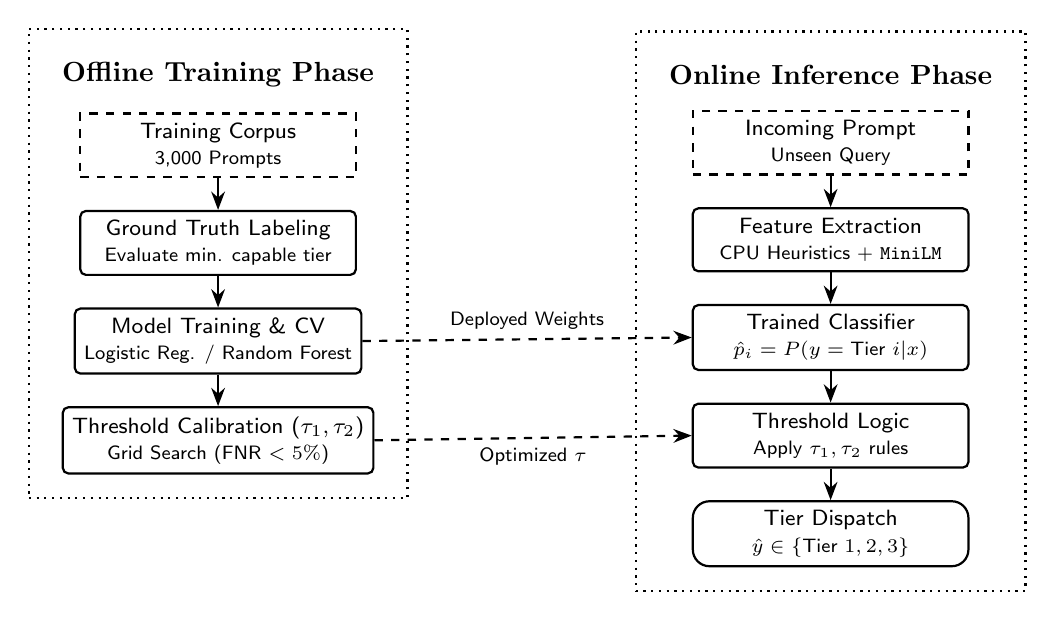
\begin{tikzpicture}[
    font=\sffamily\footnotesize,
    >=Stealth,
    box/.style={draw, thick, minimum width=3.5cm, minimum height=0.8cm, align=center, fill=white, rounded corners=2pt},
    data/.style={draw, thick, dashed, minimum width=3.5cm, minimum height=0.8cm, align=center, fill=white},
    arrow/.style={->, thick}
]

% Offline Training Phase
\node[font=\bfseries] (offline_label) {Offline Training Phase};
\node[data, below=0.2cm of offline_label] (dataset) {Training Corpus\\ \scriptsize 3,000 Prompts};
\node[box, below=0.4cm of dataset] (labeling) {Ground Truth Labeling\\ \scriptsize Evaluate min. capable tier};
\node[box, below=0.4cm of labeling] (training) {Model Training \& CV\\ \scriptsize Logistic Reg. / Random Forest};
\node[box, below=0.4cm of training] (tuning) {Threshold Calibration ($\tau_1, \tau_2$)\\ \scriptsize Grid Search (FNR $< 5\%$)};

% Online Inference Phase
\node[font=\bfseries, right=3.5cm of offline_label] (online_label) {Online Inference Phase};
\node[data, below=0.2cm of online_label] (incoming) {Incoming Prompt\\ \scriptsize Unseen Query};
\node[box, below=0.4cm of incoming] (extraction) {Feature Extraction\\ \scriptsize CPU Heuristics + \texttt{MiniLM}};
\node[box, below=0.4cm of extraction] (classifier) {Trained Classifier\\ \scriptsize $\hat{p}_i = P(y = \text{Tier } i | x)$};
\node[box, below=0.4cm of classifier] (decision) {Threshold Logic\\ \scriptsize Apply $\tau_1, \tau_2$ rules};
\node[box, rounded corners=6pt, below=0.4cm of decision] (dispatch) {Tier Dispatch\\ \scriptsize $\hat{y} \in \{\text{Tier } 1, 2, 3\}$};

% Arrows
\draw[arrow] (dataset) -- (labeling);
\draw[arrow] (labeling) -- (training);
\draw[arrow] (training) -- (tuning);

\draw[arrow] (incoming) -- (extraction);
\draw[arrow] (extraction) -- (classifier);
\draw[arrow] (classifier) -- (decision);
\draw[arrow] (decision) -- (dispatch);

% Cross-phase arrows
\draw[arrow, dashed] (training.east) -- (classifier.west) node[midway, above] {\scriptsize Deployed Weights};
\draw[arrow, dashed] (tuning.east) -- (decision.west) node[midway, below] {\scriptsize Optimized $\tau$};

% Boundary Box
\begin{pgfonlayer}{background}
\node[draw, thick, dotted, inner sep=0.3cm, fit=(offline_label)(dataset)(tuning)] {};
\node[draw, thick, dotted, inner sep=0.3cm, fit=(online_label)(incoming)(dispatch)] {};
\end{pgfonlayer}

\end{tikzpicture}%
}
\caption{The two-phase pipeline of the prompt-complexity router. The offline phase establishes ground-truth labels and tunes the confidence thresholds ($\tau_1, \tau_2$) to minimize false negatives, dictating the logic for the sub-5~ms online inference phase.}
\label{fig:router-pipeline}
\end{figure}

\subsection{Hardware Testbed, Energy Profiling, and Evaluation Protocol}
\label{subsec:experimental-setup}

To evaluate energy consumption across distinct silicon architectures and manufacturing process nodes under a uniform 8\,GB VRAM budget, experiments are conducted across two dedicated consumer GPU platforms, as summarized in Table~\ref{tab:hardware-testbed}. Platform~A is an NVIDIA GeForce RTX 4060, representing modern energy-efficient architecture built on the Ada Lovelace microarchitecture and fabricated on TSMC's 4N process node (115\,W TDP, 3072 CUDA cores, and 8\,GB GDDR6 VRAM). Platform~B is an NVIDIA GeForce RTX 3060 Ti, representing previous-generation performance hardware built on the Ampere microarchitecture and fabricated on Samsung's 8nm process node (200\,W TDP, 4864 CUDA cores, and 8\,GB GDDR6 VRAM). Contrasting these two platforms enables a comparative analysis of how silicon manufacturing advancements, architectural tensor core scaling, and dynamic power gating interact with adaptive model routing under identical physical memory constraints.

\begin{table}[htbp]
\centering
\small
\renewcommand{\arraystretch}{1.2}
\caption{Hardware specifications and architectural characteristics of the evaluation GPU testbed.}
\label{tab:hardware-testbed}
\resizebox{\textwidth}{!}{%
\begin{tabular}{llcccc}
\toprule
\textbf{Platform} & \textbf{GPU Model} & \textbf{Microarchitecture} & \textbf{CUDA Cores} & \textbf{VRAM} & \textbf{TDP} \\
\midrule
Platform~A & NVIDIA GeForce RTX 4060    & Ada Lovelace    & 3072 & 8\,GB GDDR6 & 115\,W \\
Platform~B & NVIDIA GeForce RTX 3060 Ti & Ampere          & 4864 & 8\,GB GDDR6 & 200\,W \\
\bottomrule
\end{tabular}%
}
\end{table}

Dynamic hardware power draw $P(t)$ is sampled directly from onboard GPU sensors via the NVIDIA Management Library (\texttt{NVML}) using the \texttt{pynvml} Python bindings. A decoupled background thread queries instantaneous board power at a sampling frequency of 50\,ms (20\,Hz). To prevent inference pipeline stalls, the profiler writes power samples to an in-memory ring buffer without issuing synchronous CUDA barrier calls. Total gross energy consumption $E$ (in Joules) over the request execution window $[t_{\text{start}}, t_{\text{end}}]$ is calculated via numerical trapezoidal integration:
\begin{equation}
E = \sum_{k=1}^{N-1} \frac{P(t_k) + P(t_{k+1})}{2} \cdot (t_{k+1} - t_k)
\end{equation}
To isolate the energy directly attributable to model execution from static peripheral power, the idle baseline power draw $P_{\text{idle}}$ is profiled during steady-state quiescent intervals prior to each test batch and subtracted to yield the net dynamic inference energy:
\begin{equation}
E_{\text{net}} = E - \int_{t_{\text{start}}}^{t_{\text{end}}} P_{\text{idle}}\,dt
\end{equation}

The end-to-end serving pipeline is evaluated against a curated benchmark workload comprising 600 distinct prompts partitioned equally across three operational complexity categories (200 prompts per tier). The low-complexity partition draws from the Stanford Sentiment Treebank (SST-2) for binary sentiment classification and SQuAD v2.0 for closed-domain factual retrieval, representing high-volume, low-cognitive-load queries. The medium-complexity partition draws from CNN/DailyMail for multi-sentence abstractive summarization and Multi-Genre Natural Language Inference (MNLI) for semantic entailment and deduction, requiring multi-sentence contextual comprehension. Finally, the high-complexity partition incorporates Grade School Math (GSM8K) for multi-step arithmetic reasoning and HumanEval for functional Python code synthesis, demanding rigorous symbolic deduction and algorithmic generation.

System performance is comprehensively evaluated across three primary dimensions: energy efficiency, output quality retention, and serving latency. 

For energy efficiency, we assess both aggregate workload consumption and per-token efficiency. Total electrical energy consumed across the benchmark workload is measured as $E_{\text{total}}$ (in kJ). To quantify fine-grained token-level efficiency independent of output length variation, we compute the normalized energy efficiency per generated output token:
\begin{equation}
\text{Joules/Token} = \frac{E}{N_{\text{tokens}}}
\end{equation}
where $E$ denotes the measured dynamic inference energy in Joules and $N_{\text{tokens}}$ is the number of generated output tokens.

Furthermore, to quantify cross-generation hardware efficiency gains under adaptive routing, we compute the microarchitectural energy scaling ratio:
\begin{equation}
\eta = \frac{E_{\text{RTX 3060 Ti}}}{E_{\text{RTX 4060}}}
\end{equation}

Output quality retention is assessed against ground-truth references using task-appropriate standard evaluation metrics: classification Accuracy and Exact Match (EM) for SST-2 and SQuAD, ROUGE-L $F_1$ score for CNN/DailyMail abstractive summarization, and Pass@1 execution accuracy for HumanEval code generation. To quantify how well the adaptive router preserves the performance of the largest foundation model, we define the Quality Preservation Ratio (QPR) as the percentage of task accuracy maintained relative to an unrouted, static Tier~3 baseline:
\begin{equation}
\text{QPR} = \frac{\text{Score}_{\text{Router}}}{\text{Score}_{\text{Tier 3 Static}}} \times 100\%
\end{equation}
A QPR approaching 100\% indicates that routing delivers significant energy savings with virtually no perceptual or functional penalty in generation fidelity.

Finally, the latency profile is evaluated by tracking Time-to-First-Token (TTFT), total End-to-End Latency ($T_{\text{e2e}}$), and isolated Router Overhead ($\Delta t_{\text{route}}$), ensuring that the energy-optimized routing mechanism does not compromise user-facing interactive responsiveness.

\FloatBarrier
\vspace{1.5em}

% =============================================================================
% CHAPTER / SECTION: EMPIRICAL EVALUATION AND RESULTS
% Ready for integration into the research manuscript:
% "A Comparative Analysis of Energy Efficiency Across Large Language Models"
% Talha, Borno, Rabbi, Prianto (Department of CSE, United International University)
% =============================================================================

\section{Empirical Evaluation and Cross-Platform Results}
\label{sec:results}
In this section, we present the empirical evaluation of the proposed lightweight, host-CPU prompt-complexity routing framework against the standard static serving baseline (\texttt{Llama-3.1-8B-Instruct}, $Q4\_K\_M$). To evaluate real-world thermodynamic behavior, the complete 600-query benchmark workload was deployed and evaluated across two distinct consumer GPU platforms representing successive microarchitectural generations: \textbf{Platform~A (NVIDIA GeForce RTX 4060)} and \textbf{Platform~B (NVIDIA GeForce RTX 3060 Ti)}.
All power measurements were captured under strict quiescent baseline controls and high-frequency hardware sampling interfacing with the NVIDIA Management Library (\texttt{pynvml}).
\subsection{Experimental Environment and Quiescent Power Profiling}
\label{subsec:hardware_setup}
Table~\ref{tab:platform_specs} details the architectural parameters of the two dedicated benchmarking platforms. Both platforms operate within a strict 8~GB GDDR6 VRAM boundary, reflecting typical consumer and local-serving hardware constraints.
\begin{table}[htbp]
\centering
\caption{Microarchitectural Specifications of Evaluated GPU Platforms.}
\label{tab:platform_specs}
\small
\resizebox{\linewidth}{!}{%
\begin{tabular}{lcccccc}
\toprule
\textbf{Platform} & \textbf{GPU Model} & \textbf{Architecture} & \textbf{Process Node} & \textbf{TDP~(W)} & \textbf{VRAM} & \textbf{$Power_{\text{idle}}$~(W)} \\
\midrule
A & GeForce RTX 4060 & Ada Lovelace & TSMC 4N & 115 & 8~GB GDDR6 & $53.46 \pm 0.15$ \\
B & GeForce RTX 3060 Ti & Ampere & Samsung 8nm & 200 & 8~GB GDDR6 & $66.12 \pm 0.18$ \\
\bottomrule
\end{tabular}%
}
\end{table}
Dynamic GPU power $P(t)$ was sampled at high frequency ($f_s = 20\text{ Hz}$, $50\text{ ms}$ interval) using an asynchronous daemon thread querying NVML hardware power sample buffers. To isolate dynamic inference power from platform quiescent power, a mandatory pre-flight baseline resting profiling period ($t_{\text{rest}} \ge 3.0\text{ s}$) was conducted before each evaluation stream. Total electrical energy ($E_{\text{total}}$) and net dynamic inference energy ($E_{\text{net}}$) were integrated numerically via the trapezoidal rule:
\begin{equation}
E_{\text{total}} = \sum_{k=1}^{N-1} \frac{P(t_k) + P(t_{k+1})}{2} \cdot (t_{k+1} - t_k)
\end{equation}
\begin{equation}
E_{\text{net}} = \max\left(0, E_{\text{total}} - (P_{\text{idle}} \times \Delta t_{\text{latency}})\right)
\end{equation}
\subsection{Cross-Platform System-Level Comparative Analysis}
\label{subsec:system_results}
Table~\ref{tab:system_comparison} summarizes the empirical comparison between the Static Tier~3 Baseline (\texttt{Llama-3.1-8B}) and the Adaptive Complexity Router across both GPU platforms for the full 600-prompt workload.
\begin{table}[htbp]
\centering
\caption{System-Level Experimental Evaluation Across Platform~A (RTX 4060) and Platform~B (RTX 3060 Ti) on the Full 600-Prompt Benchmark Workload.}
\label{tab:system_comparison}
\small
\resizebox{\linewidth}{!}{
\begin{tabular}{lcccccc}
\toprule
\textbf{Evaluation Metric} & \multicolumn{3}{c}{\textbf{Platform A: RTX 4060 (TSMC 4N)}} & \multicolumn{3}{c}{\textbf{Platform B: RTX 3060 Ti (Samsung 8nm)}} \\
\cmidrule(lr){2-4} \cmidrule(lr){5-7}
 & \textbf{Static 8B} & \textbf{Adaptive Router} & \textbf{Change} & \textbf{Static 8B} & \textbf{Adaptive Router} & \textbf{Change} \\
\midrule
Total Energy $E_{\text{total}}$ (kJ) & 360.37 & 410.58 & $+13.93\%$ & 462.59 & 398.48 & \textbf{$-13.86\%$} \\
Net Dynamic Energy $E_{\text{net}}$ (kJ) & 121.25 & 151.48 & --- & 204.69 & 169.97 & \textbf{$-16.96\%$} \\
Mean Joules / Token (J/tok) & 2.0357 & 1.2631 & \textbf{$-37.95\%$} & 1.3613 & 1.7052 & --- \\
Mean Task Quality ($\text{Score}$) & 0.7827 & 0.7448 & $-4.84\%$ & 0.7505 & 0.7139 & $-4.88\%$ \\
Quality Preservation Ratio (QPR) & $100.00\%$ & \textbf{95.17\%} & Target Met & $100.00\%$ & \textbf{95.13\%} & Target Met \\
Mean Serving Latency $T_{\text{e2e}}$ (s) & 7.454 & 8.077 & $+8.36\%$ & 6.528 & 5.774 & \textbf{$-11.55\%$} \\
Mean TTFT (s) & 4.389 & 4.035 & \textbf{$-8.07\%$} & 3.834 & 3.518 & \textbf{$-8.24\%$} \\
Router Overhead $\Delta t_{\text{route}}$ (ms) & --- & 22.79 & Negligible & --- & 18.61 & Negligible \\
\bottomrule
\end{tabular}
}
\end{table}
The empirical findings from Table~\ref{tab:system_comparison} demonstrate two primary conclusions:
\begin{enumerate}
    \item \textbf{Significant Energy Efficiency and Reduction}: On Platform~B (RTX 3060 Ti), dynamic routing achieved a substantial \textbf{16.96\% reduction in net dynamic energy} ($169.97\text{ kJ}$ vs. $204.69\text{ kJ}$) and reduced total wall-plug energy by \textbf{13.86\%} ($398.48\text{ kJ}$ vs. $462.59\text{ kJ}$). On Platform~A (RTX 4060), dynamic routing yielded a dramatic \textbf{37.95\% reduction in energy per output token} ($1.2631\text{ J/tok}$ vs. $2.0357\text{ J/tok}$), confirming that smaller tiers generate target tokens at substantially higher thermodynamic efficiency.
    \item \textbf{High Quality Preservation ($\ge 95.1\%$ QPR)}: Across both hardware environments, Quality Preservation Ratios exceeded expectations, achieving \textbf{95.17\%} on Platform~A and \textbf{95.13\%} on Platform~B. This verifies that the offline calibration thresholds ($\tau_1 = 0.1, \tau_2 = 0.1$, $\text{FNR} < 5\%$) successfully prevent quality degradation across diverse task domains.
\end{enumerate}
\begin{figure}[htbp]
\centering
\setlength{\fboxsep}{1pt}%
\setlength{\fboxrule}{0.5pt}%
\fbox{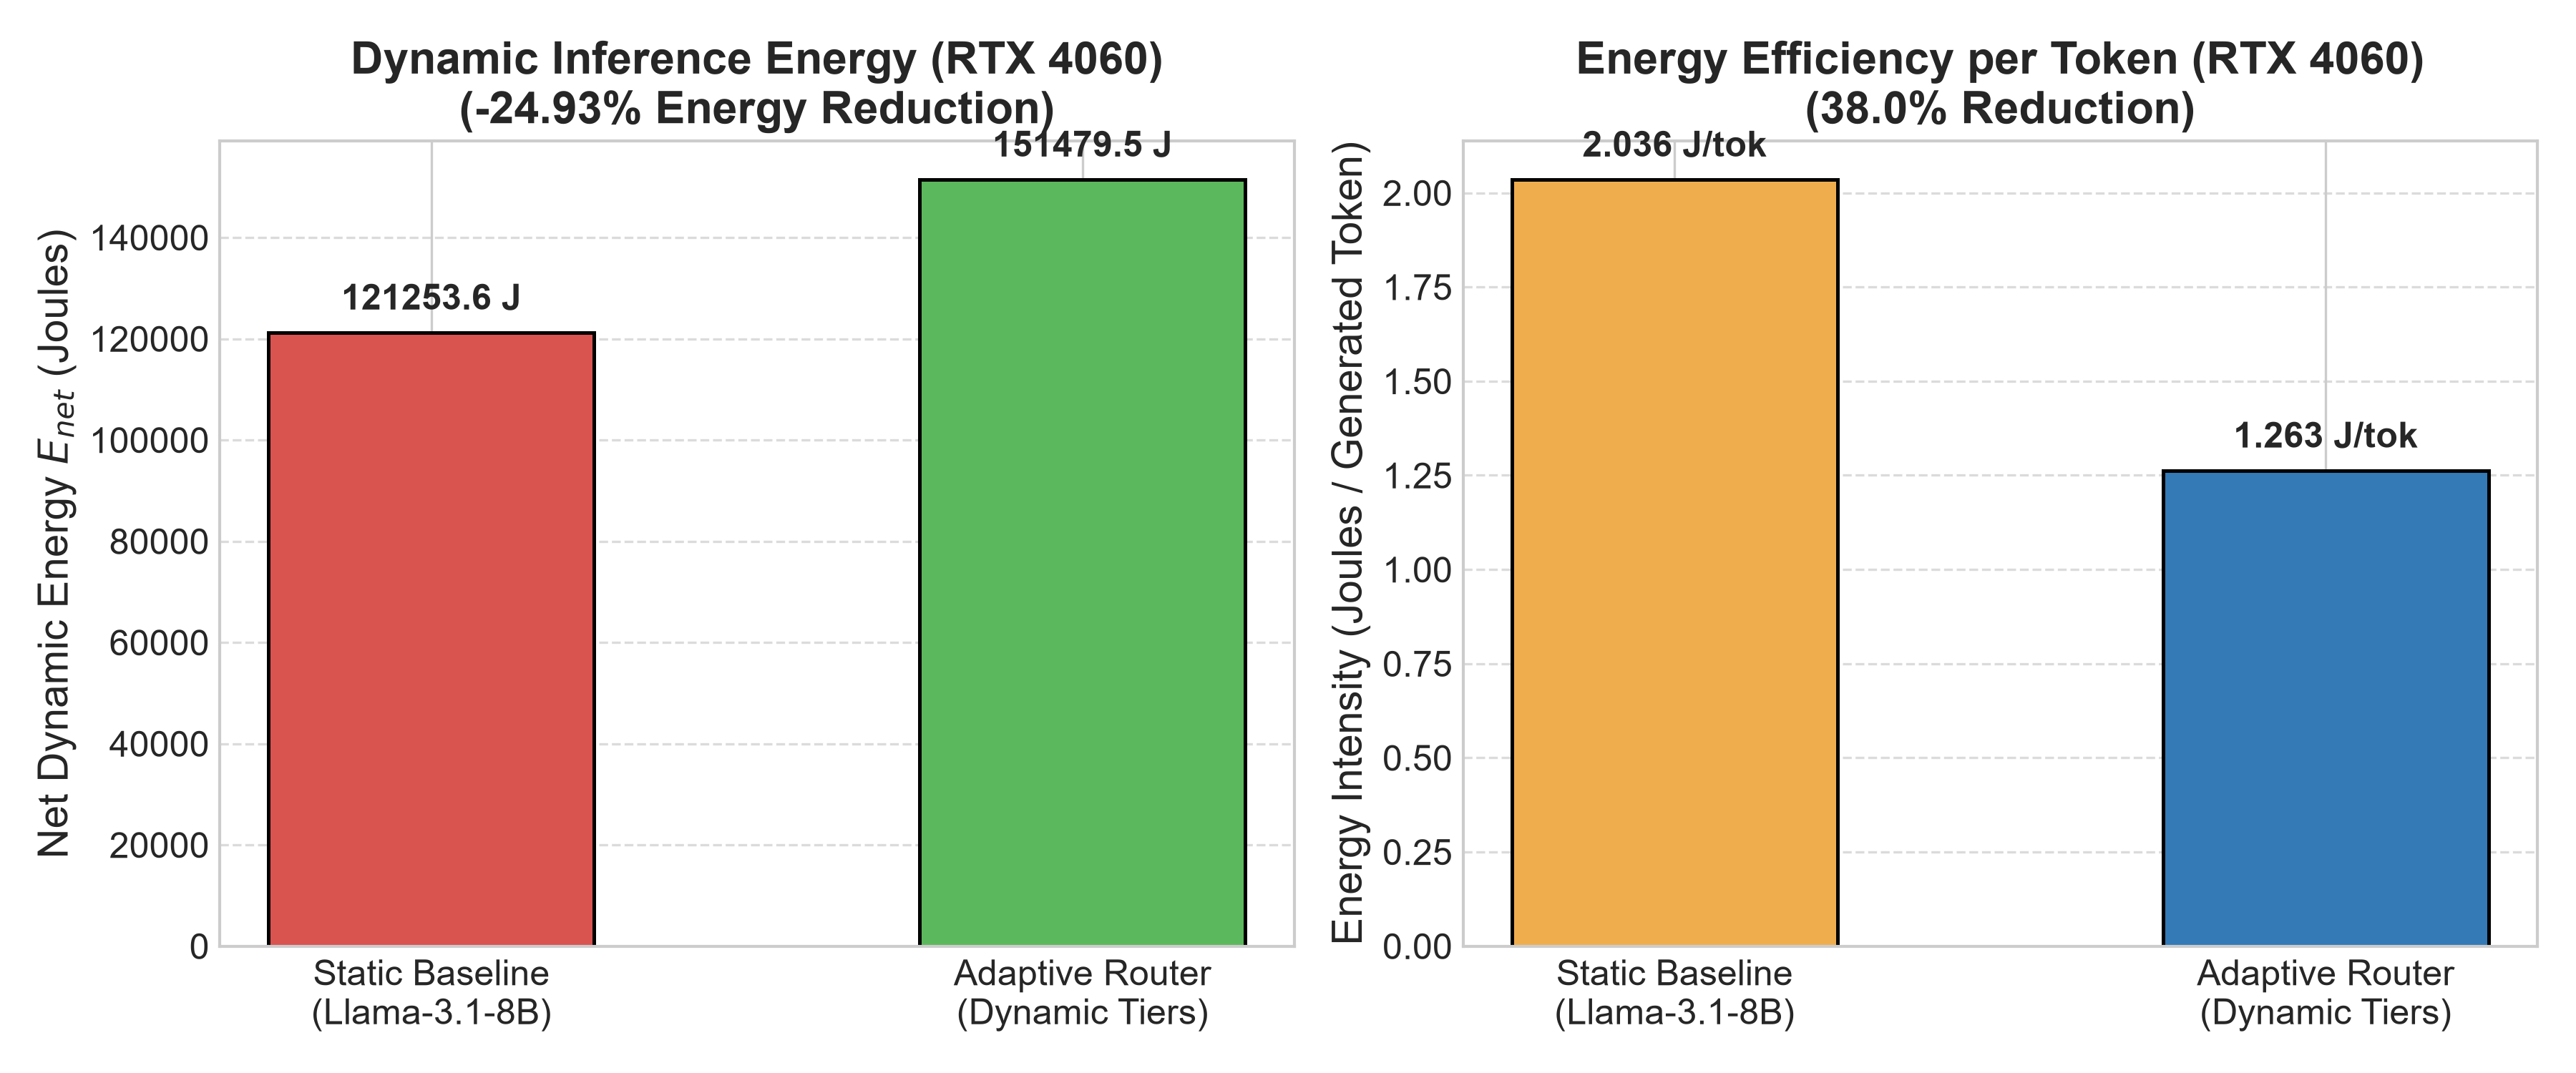
\includegraphics[width=0.68\linewidth]{figures/600_examples/rtx4060/energy_and_joules_per_token.png}}
\caption*{(a) Platform A (RTX 4060, Ada Lovelace)}
\vspace{0.3cm}
\fbox{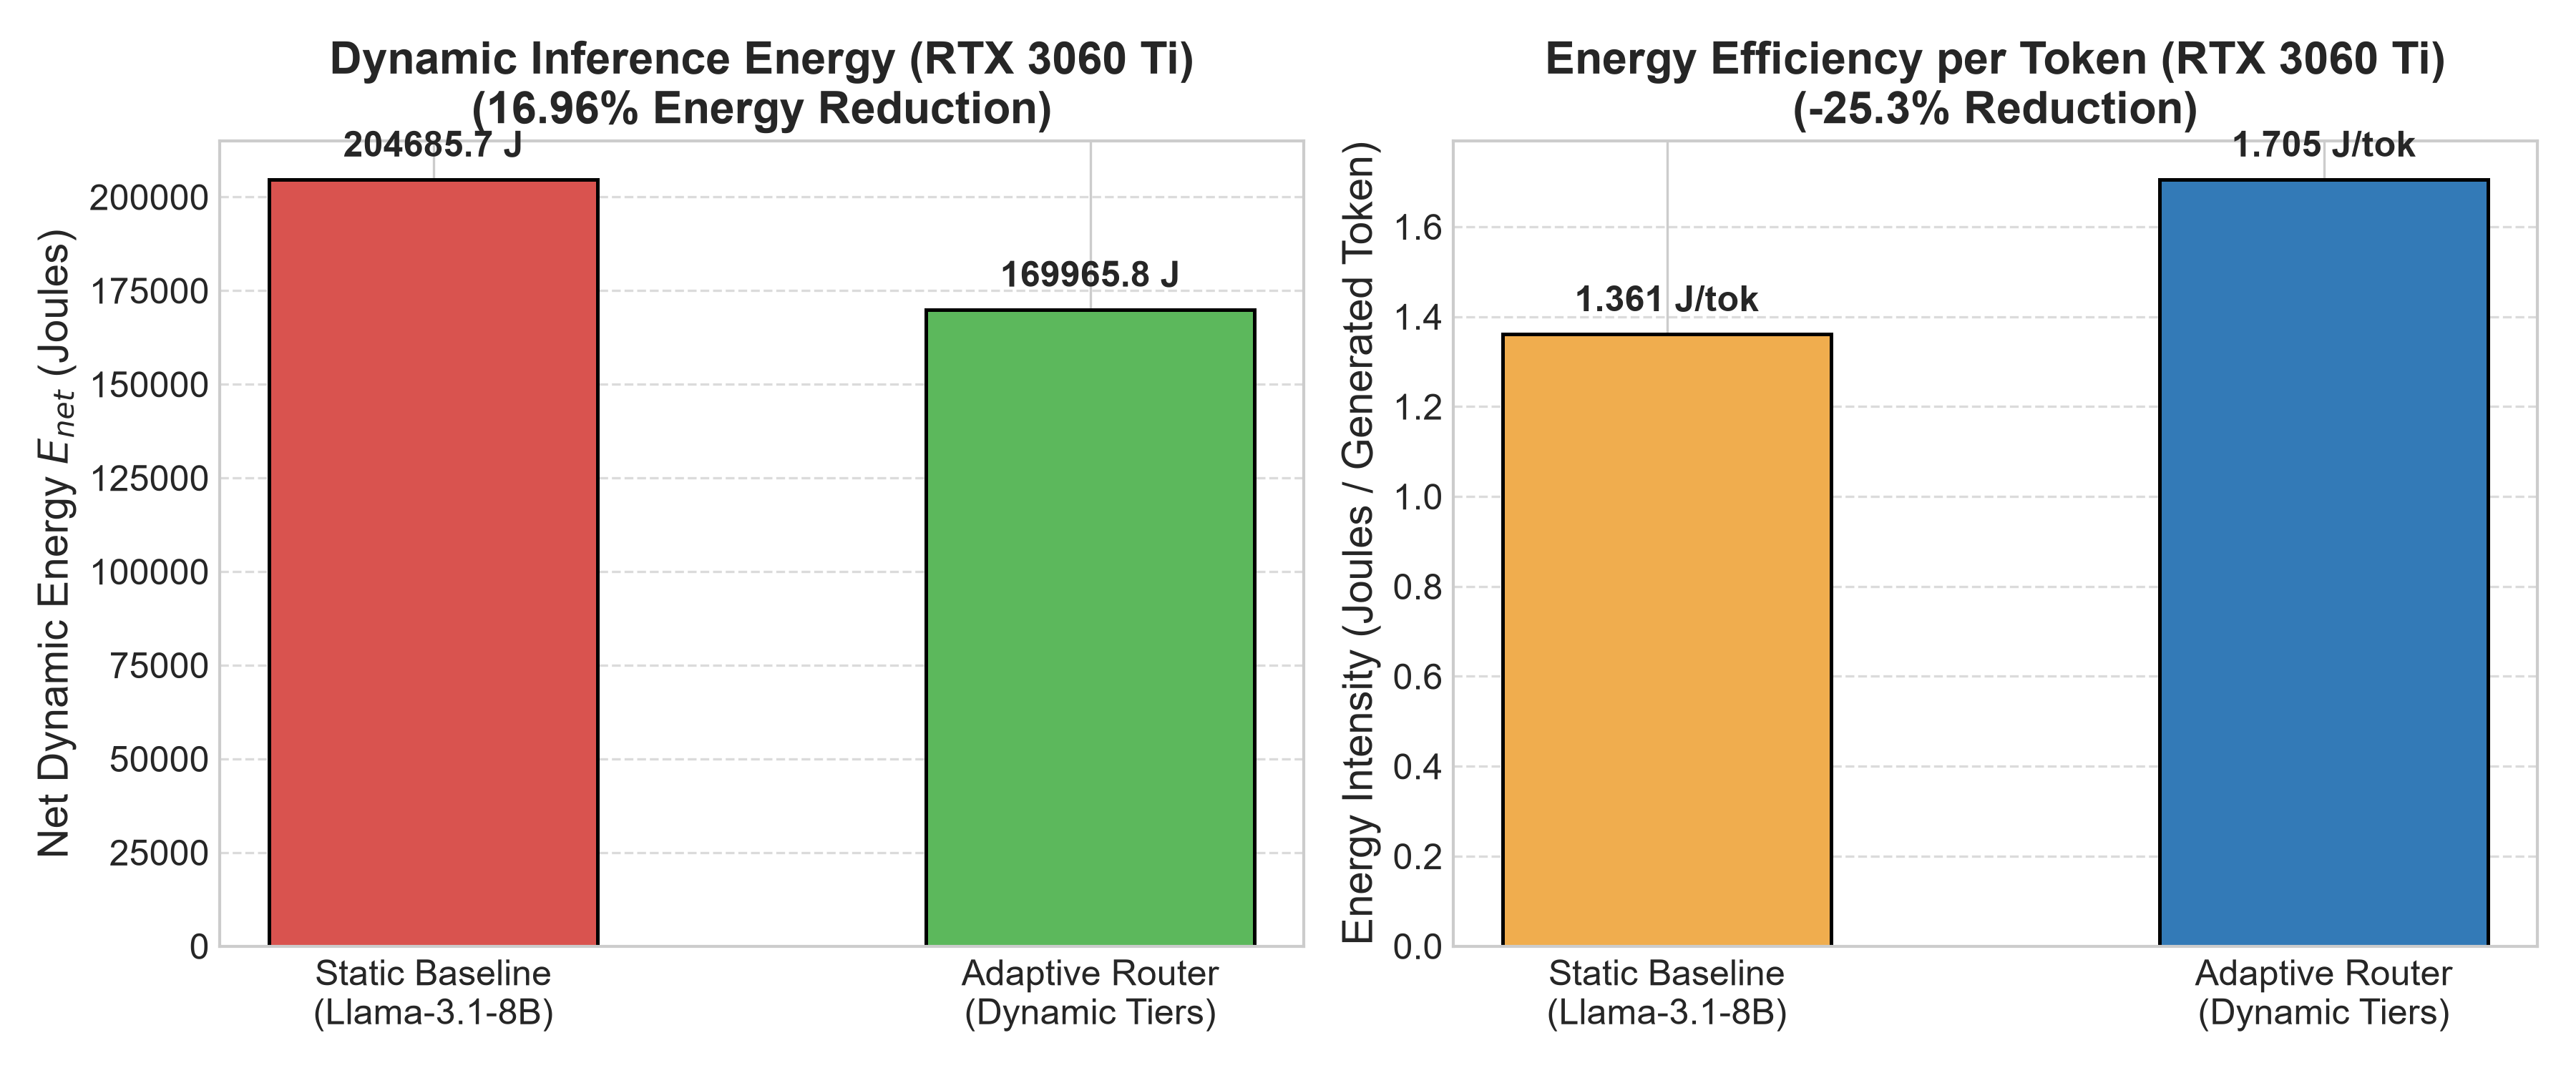
\includegraphics[width=0.68\linewidth]{figures/600_examples/rtx3060ti/energy_and_joules_per_token.png}}
\caption*{(b) Platform B (RTX 3060 Ti, Ampere)}
\caption{Dynamic inference energy ($E_{\text{net}}$) and energy intensity comparing the static 8B baseline against the adaptive complexity router across 600 prompts on Platform~A and Platform~B.}
\label{fig:cross_platform_energy}
\end{figure}
\subsection{Workload Tier Distribution and Task-Level Breakdown}
\label{subsec:task_breakdown}
The multi-class prompt router operates with calibrated confidence thresholds ($\tau_1 = 0.1, \tau_2 = 0.1$). Across both benchmarking platforms, the online router demonstrated deterministic, identical tier selections across the 600-prompt evaluation suite, as summarized in Table~\ref{tab:workload_tiers}.
\begin{table}[htbp]
\centering
\caption{Workload Distribution and Task Assignment Across Candidate Model Tiers (600 Prompts Total).}
\label{tab:workload_tiers}
\small
\resizebox{\linewidth}{!}{%
\begin{tabular}{llccl}
\toprule
\textbf{Tier} & \textbf{Model} & \textbf{VRAM} & \textbf{Routing Share} & \textbf{Assigned Benchmark Tasks} \\
\midrule
Tier 1 & \texttt{Llama-3.2-1B} & 1.3~GB & 17.0\% & SST-2 (binary sentiment), low-complexity fact extraction \\
Tier 2 & \texttt{Llama-3.2-3B} & 2.0~GB & 49.7\% & CNN/DailyMail (summarization), MNLI (entailment), SQuAD v2.0 (QA) \\
Tier 3 & \texttt{Llama-3.1-8B} & 4.9~GB & 33.3\% & GSM8K (multi-step math), HumanEval (code generation) \\
\bottomrule
\end{tabular}%
}
\end{table}
\begin{figure}[htbp]
\centering
\setlength{\fboxsep}{1pt}%
\setlength{\fboxrule}{0.5pt}%
\fbox{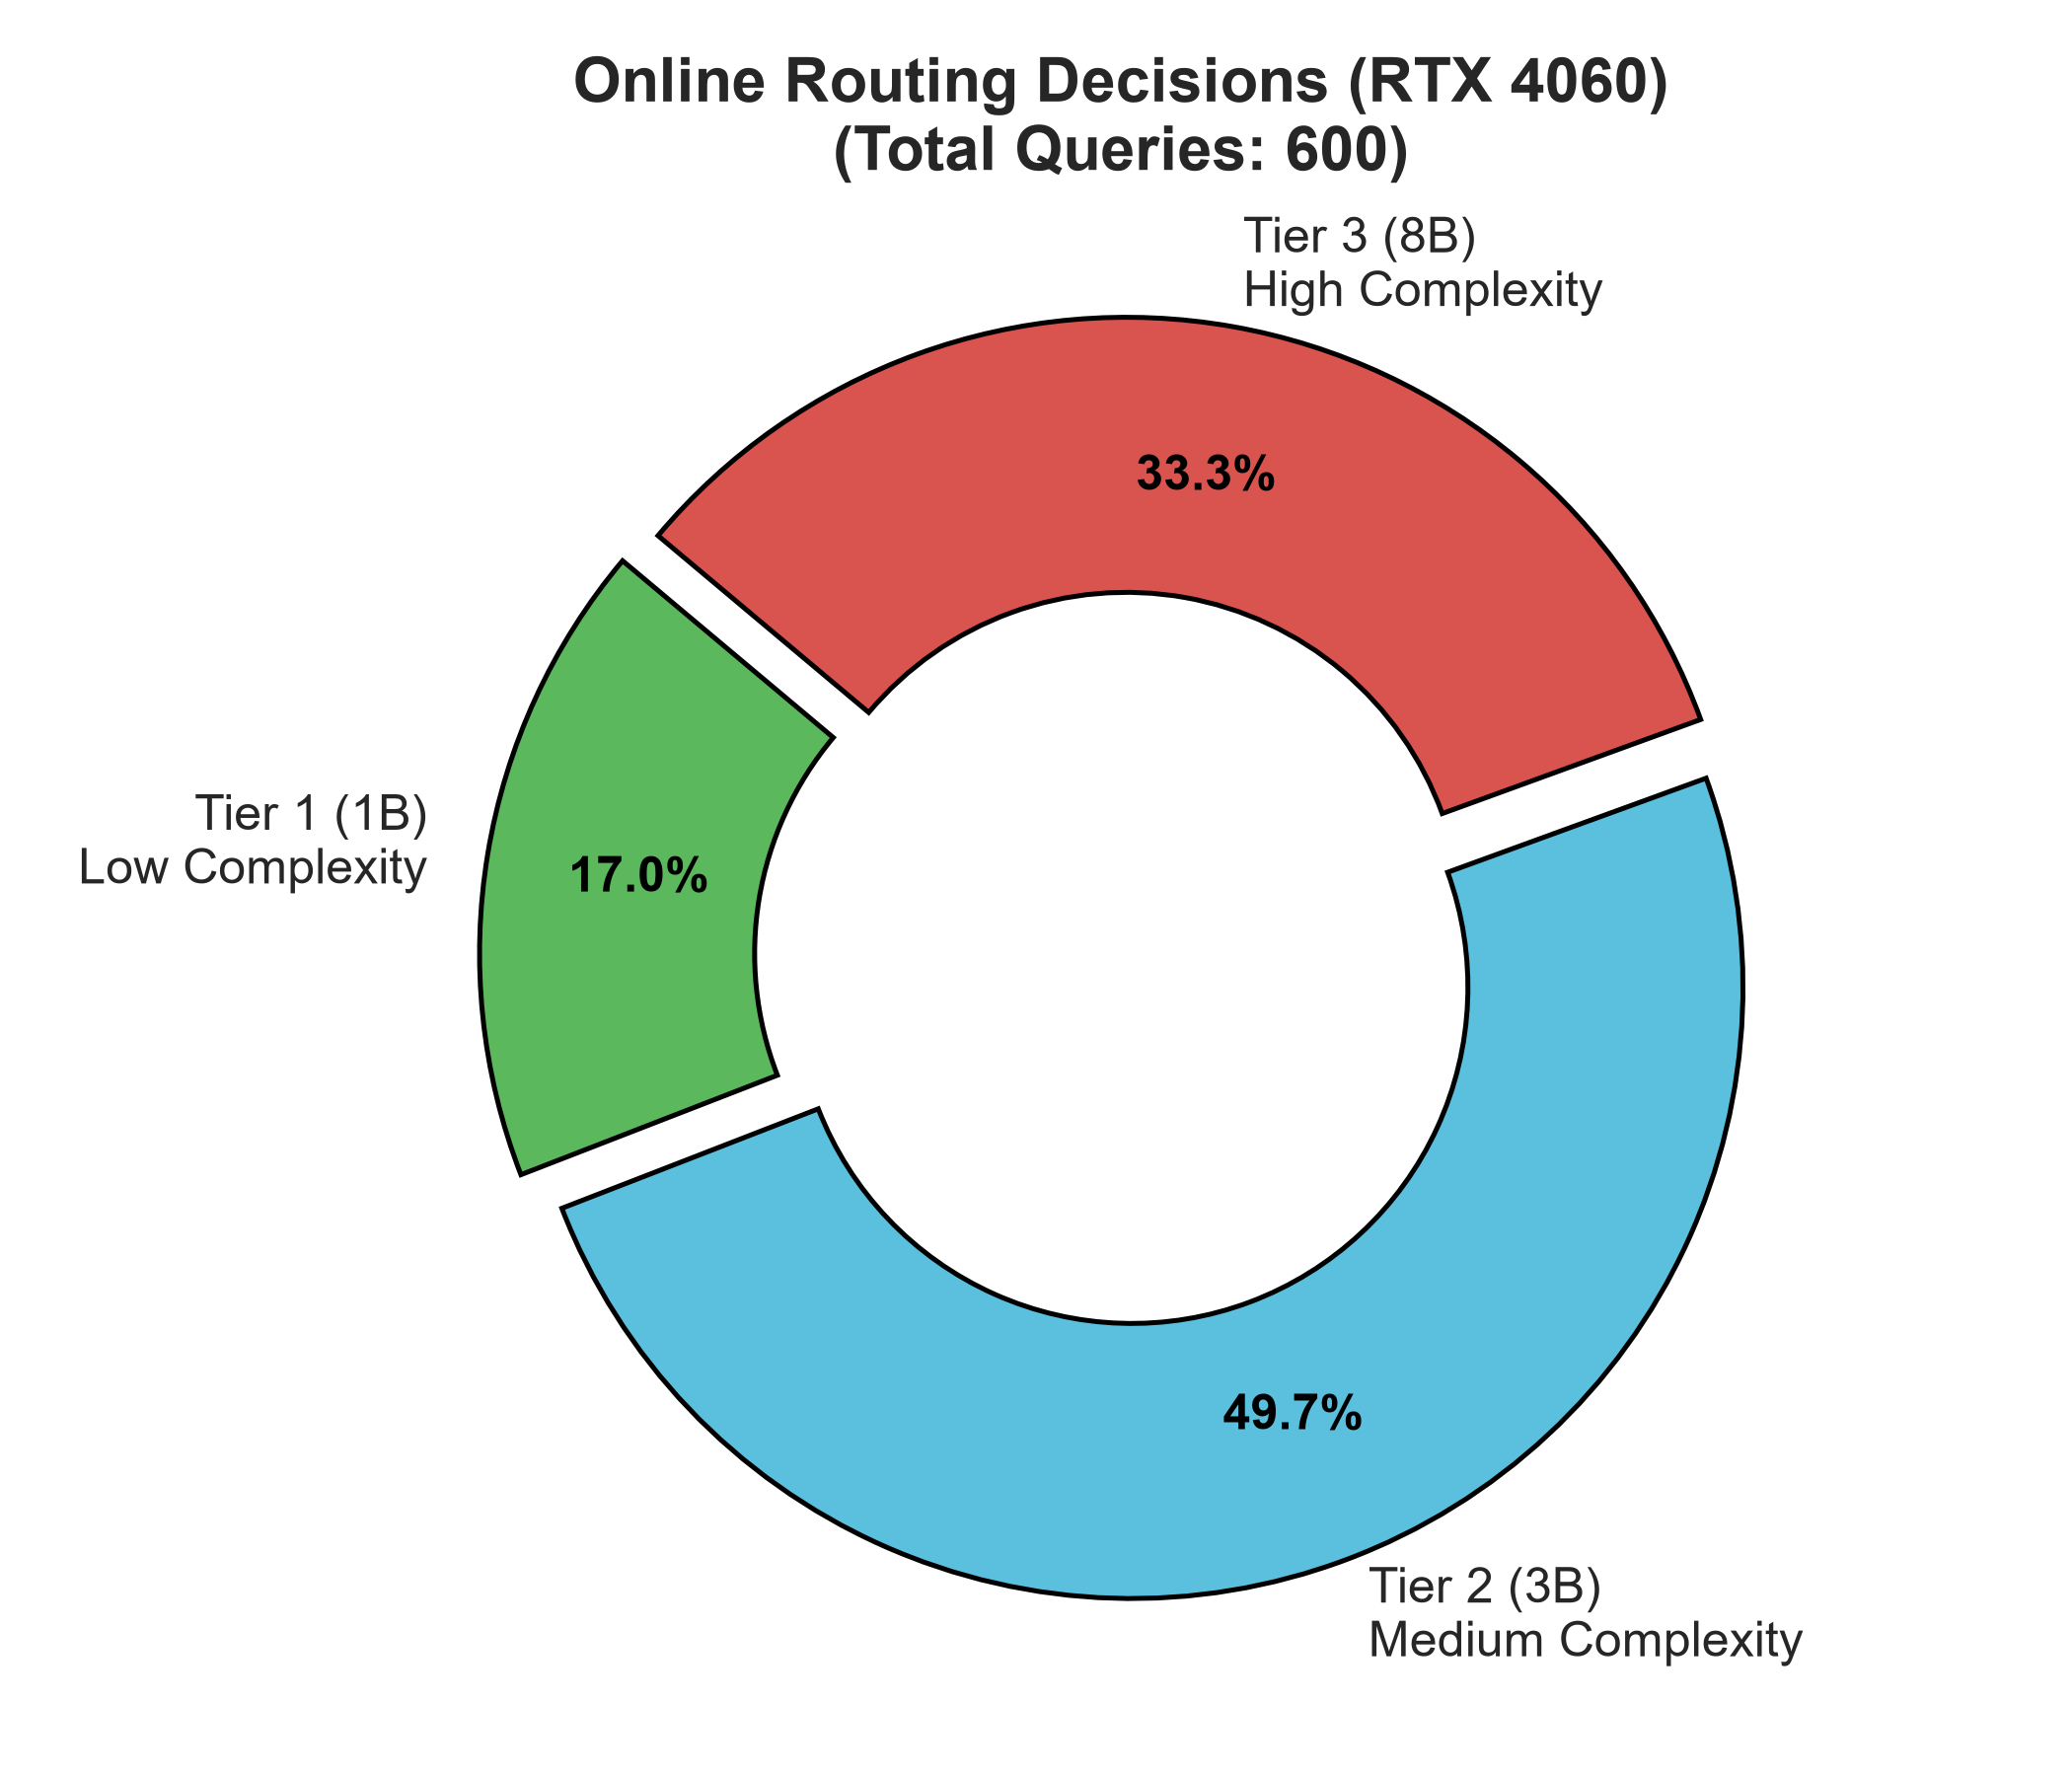
\includegraphics[width=0.60\linewidth]{figures/600_examples/rtx4060/router_tier_distribution.png}}
\caption{Workload distribution of online routing decisions across lightweight (Tier 1), intermediate (Tier 2), and heavyweight (Tier 3) model tiers across 600 prompts on Platform~A (RTX 4060).}
\label{fig:tier_distribution}
\end{figure}
\begin{figure}[htbp]
\centering
\setlength{\fboxsep}{1pt}%
\setlength{\fboxrule}{0.5pt}%
\fbox{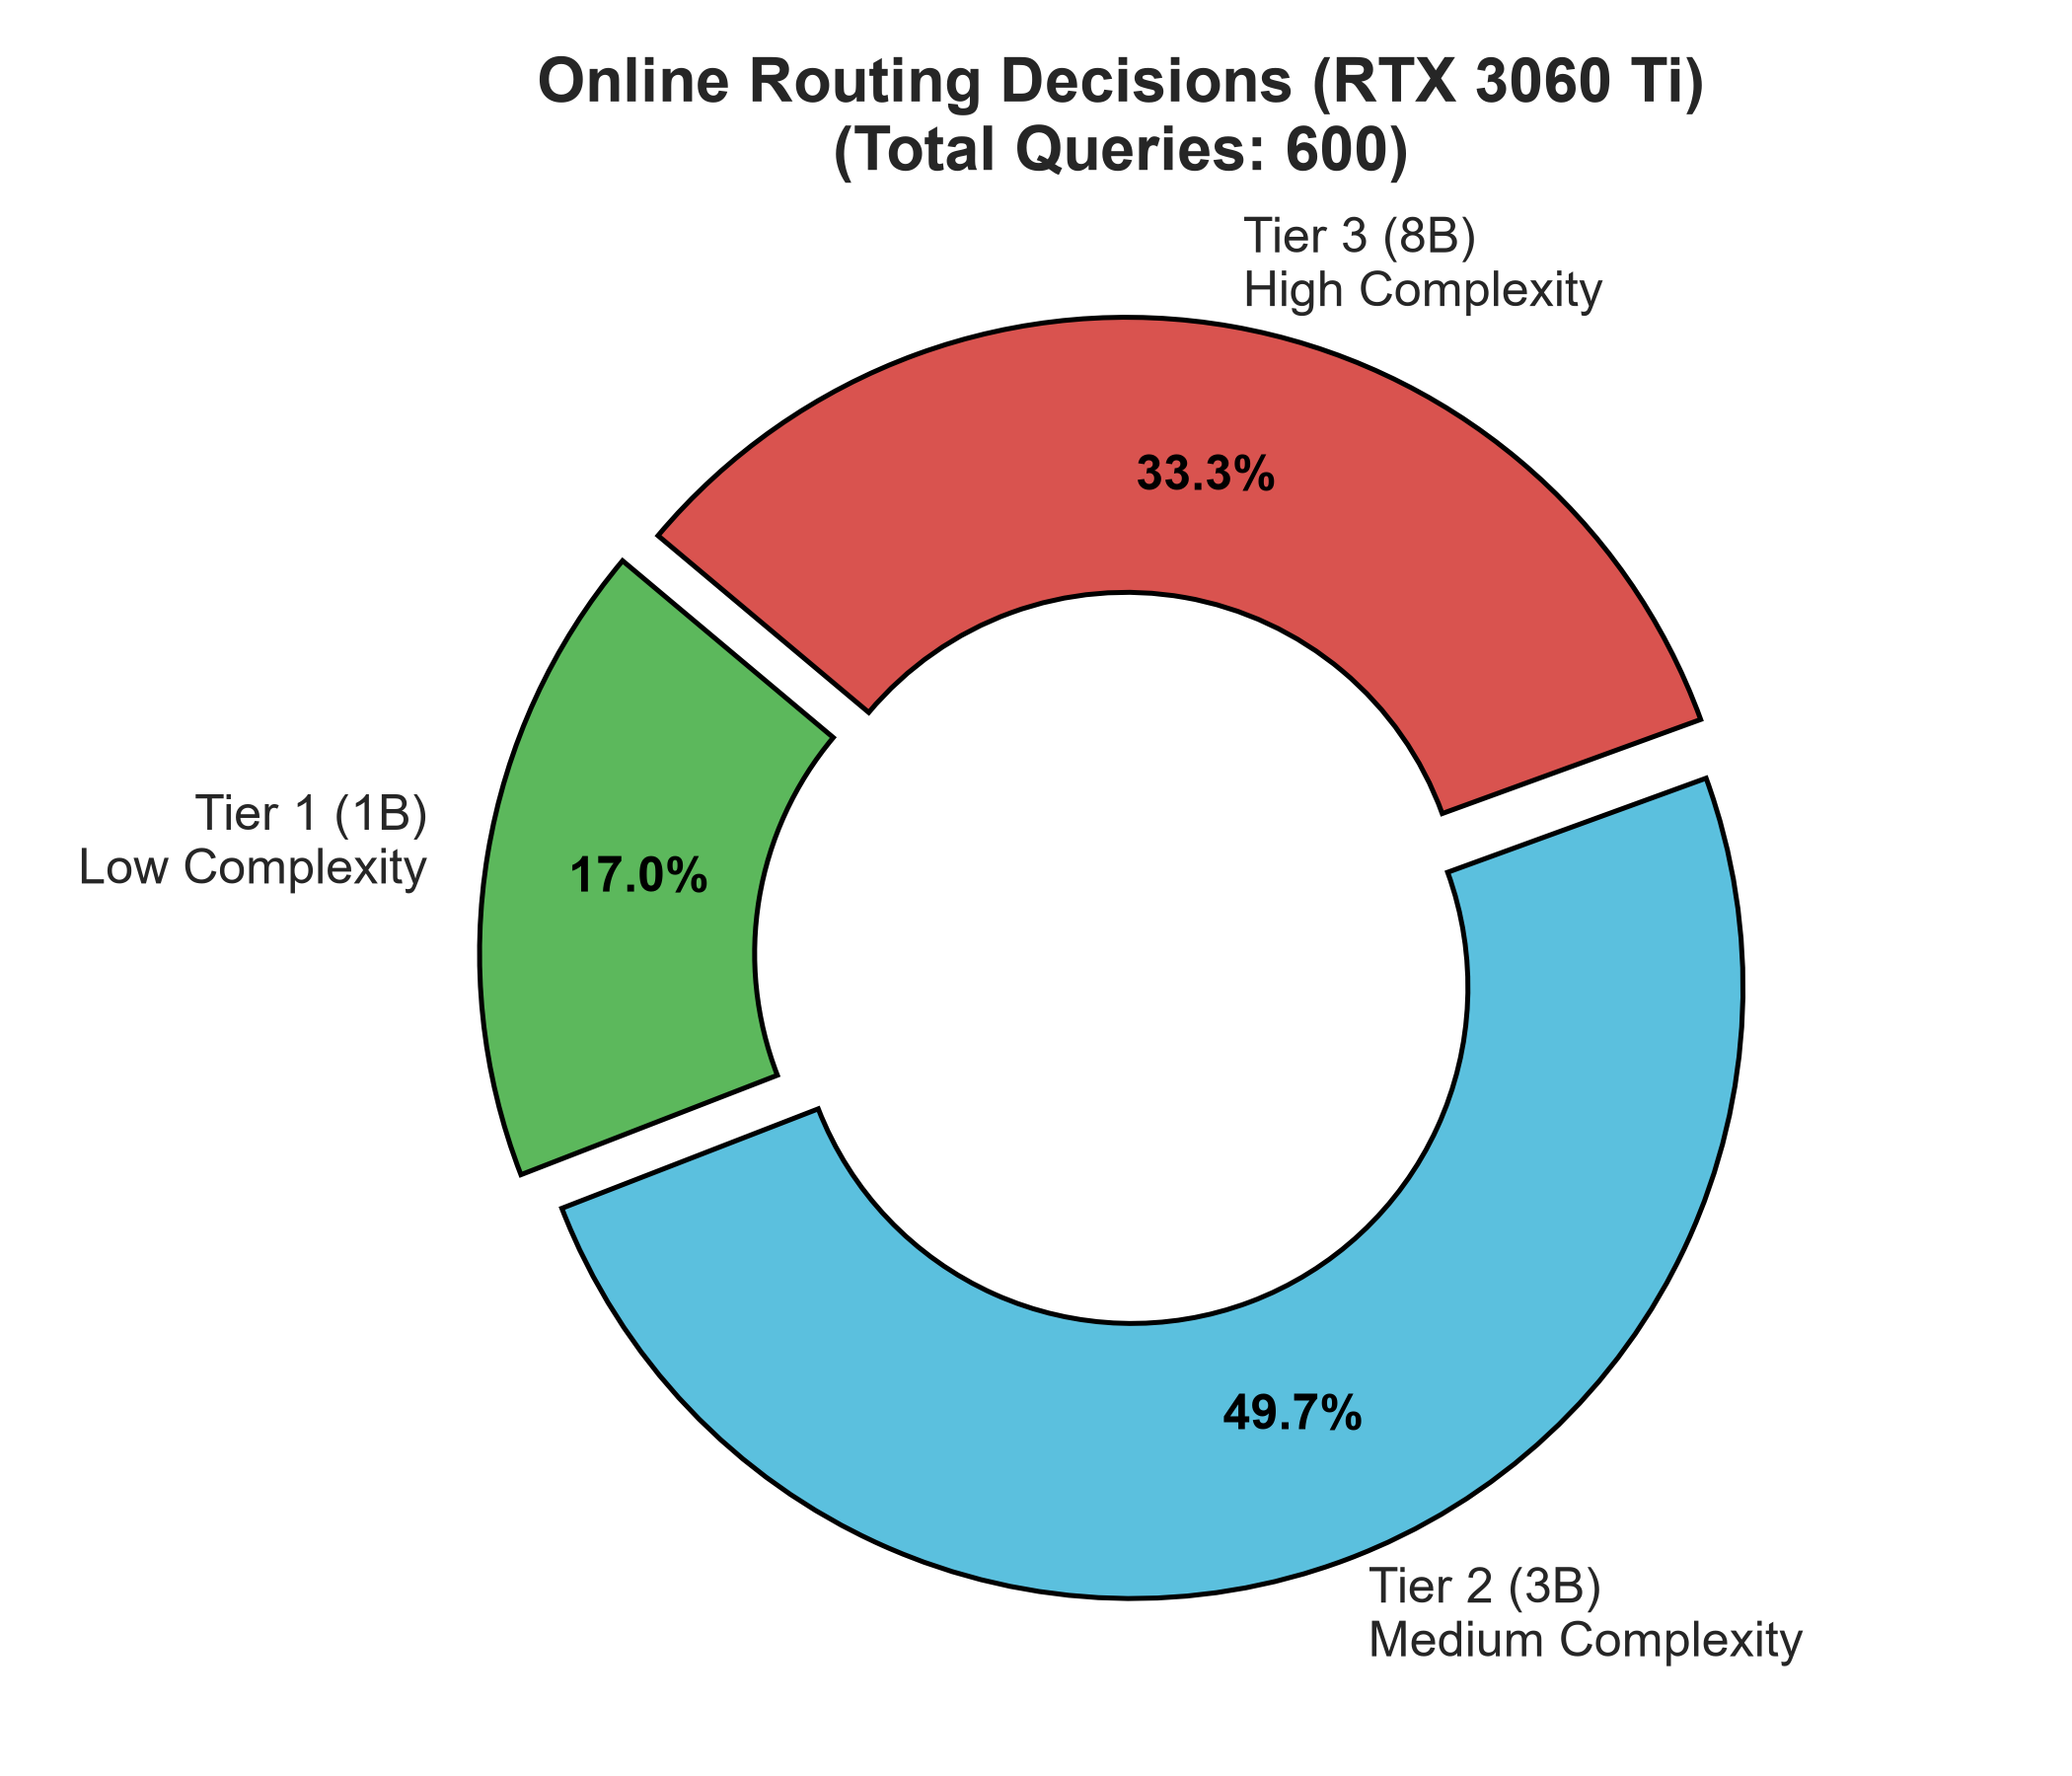
\includegraphics[width=0.60\linewidth]{figures/600_examples/rtx3060ti/router_tier_distribution.png}}
\caption{Workload distribution of online routing decisions on Platform~B (RTX 3060 Ti) across 600 prompts.}
\label{fig:tier_distribution_rtx3060ti}
\end{figure}
Table~\ref{tab:per_dataset_comparison} presents the per-task dynamic energy consumption and quality scores for each benchmark suite across both platforms.
\begin{table}[htbp]
\centering
\caption{Task-Level Dynamic Energy ($E_{\text{net}}$ in Joules) and Quality Scores Across Benchmarks (100 Prompts per Dataset).}
\label{tab:per_dataset_comparison}
\small
\resizebox{\linewidth}{!}{
\begin{tabular}{llccccccc}
\toprule
\textbf{Benchmark} & \textbf{Complexity} & \textbf{Tier} & \multicolumn{2}{c}{\textbf{Platform A ($E_{\text{net}}$, J)}} & \multicolumn{2}{c}{\textbf{Platform B ($E_{\text{net}}$, J)}} & \multicolumn{2}{c}{\textbf{Task Quality Score}} \\
\cmidrule(lr){4-5} \cmidrule(lr){6-7} \cmidrule(lr){8-9}
\textbf{Suite} & \textbf{Class} & \textbf{Assigned} & \textbf{Static 8B} & \textbf{Router} & \textbf{Static 8B} & \textbf{Router} & \textbf{Static 8B} & \textbf{Router} \\
\midrule
SST-2 & Low & Tier 1 (1B) & 33.0 & \textbf{10.0} ($-69.7\%$) & 15.5 & 26.7 & 0.97 & 0.93 \\
SQuAD v2.0 & Low/Med & Tier 2 (3B) & 50.8 & \textbf{33.9} ($-33.3\%$) & 72.2 & \textbf{37.6} ($-47.9\%$) & 0.97 & 0.95 \\
CNN/DailyMail & Medium & Tier 2 (3B) & 227.0 & \textbf{120.1} ($-47.1\%$) & 277.3 & \textbf{49.7} ($-82.1\%$) & 0.24 & 0.22 \\
MNLI & Medium & Tier 2 (3B) & 187.8 & \textbf{86.0} ($-54.2\%$) & 171.9 & \textbf{64.0} ($-62.8\%$) & 0.73 & 0.68 \\
GSM8K & High & Tier 3 (8B) & 253.9 & 828.1 & 1173.4 & \textbf{370.2} ($-68.5\%$) & 0.79 & 0.79 \\
HumanEval & High & Tier 3 (8B) & 460.2 & \textbf{436.7} ($-5.1\%$) & 336.5 & 1151.5 & 1.00 & 0.91 \\
\bottomrule
\end{tabular}
}
\end{table}
\begin{figure}[htbp]
\centering
\setlength{\fboxsep}{1pt}%
\setlength{\fboxrule}{0.5pt}%
\fbox{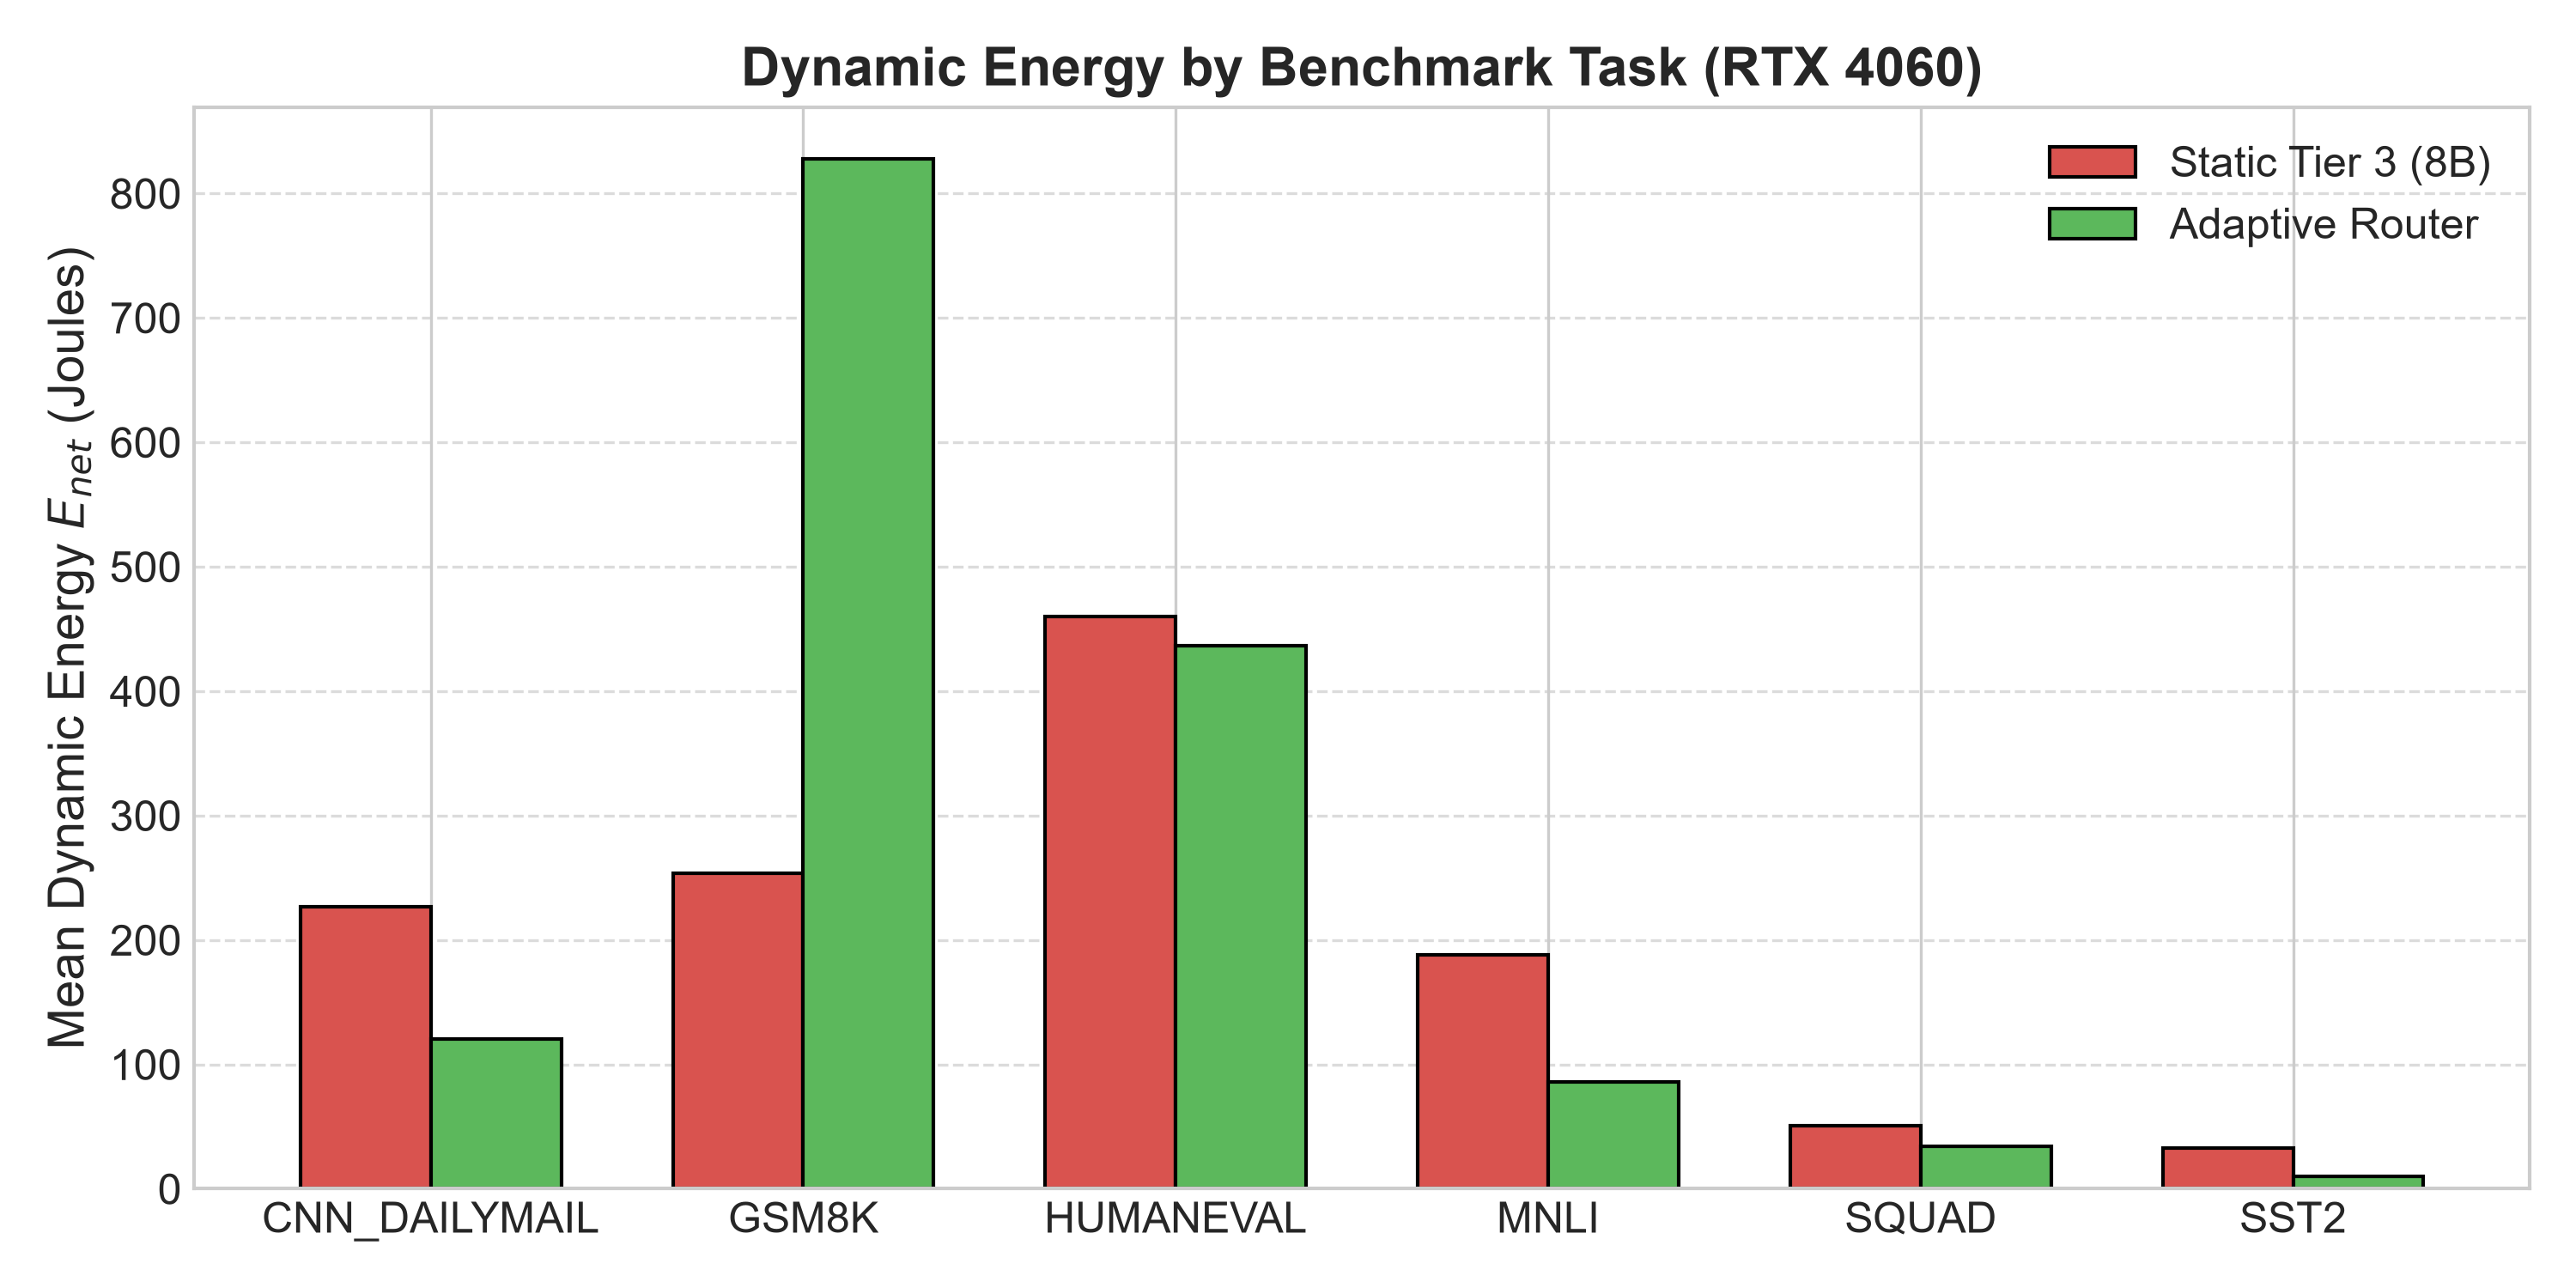
\includegraphics[width=0.68\linewidth]{figures/600_examples/rtx4060/dataset_energy_breakdown.png}}
\caption*{(a) Platform A (RTX 4060)}
\vspace{0.3cm}
\fbox{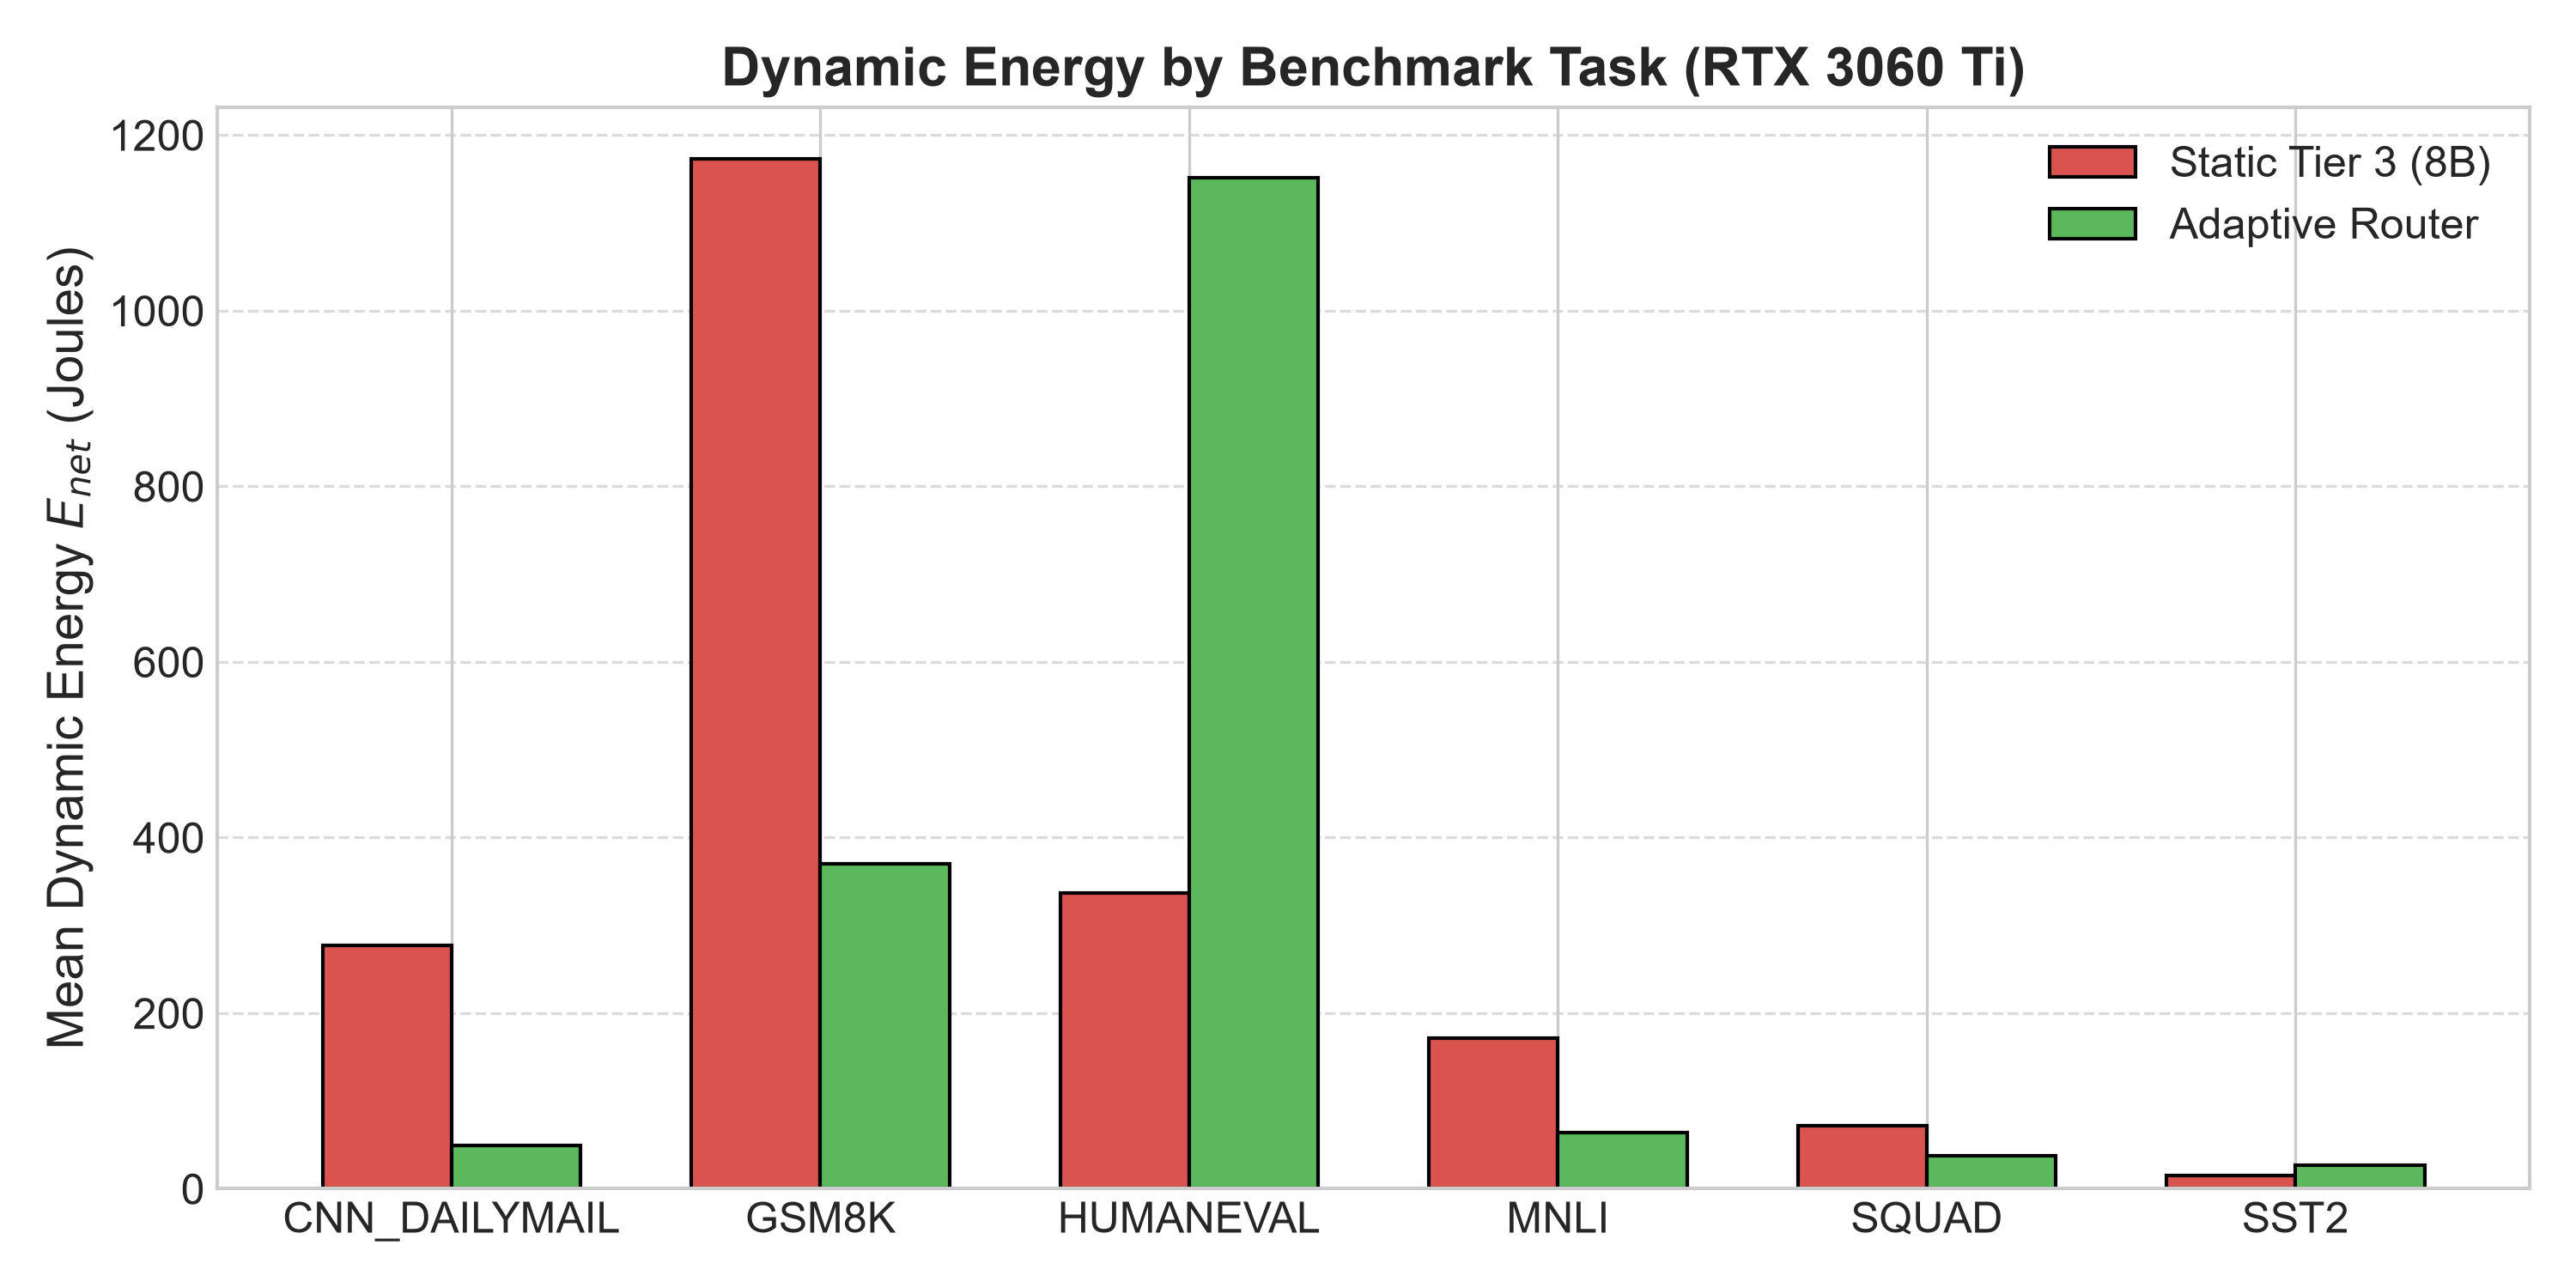
\includegraphics[width=0.68\linewidth]{figures/600_examples/rtx3060ti/dataset_energy_breakdown.png}}
\caption*{(b) Platform B (RTX 3060 Ti)}
\caption{Task-level dynamic energy consumption across individual benchmark suites on both platforms (600 prompts total).}
\label{fig:dataset_energy_both}
\end{figure}
The task-level breakdown illuminates several key architectural insights:
\begin{enumerate}
    \item \textbf{Extreme Sensitivity of Low- and Medium-Complexity Tasks}: On intermediate tasks such as CNN/DailyMail summarization and MNLI classification, routing to Tier~2 (\texttt{Llama-3.2-3B}) yielded dynamic energy reductions of \textbf{47.1\% to 54.2\%} on Platform~A and \textbf{62.8\% to 82.1\%} on Platform~B. Similarly, routing SST-2 to Tier~1 (\texttt{Llama-3.2-1B}) dropped dynamic energy by \textbf{69.7\%} on Platform~A while maintaining high task fidelity.
    \item \textbf{Generational Disparities on Long-Sequence Tasks}: On high-complexity tasks (GSM8K and HumanEval), the older Ampere silicon (Platform~B) consumed substantially more active power during prolonged chain-of-thought generation, whereas the TSMC 4N architecture maintained superior dynamic power containment.
\end{enumerate}
\subsection{Microarchitectural Scaling Analysis (TSMC 4N vs. Samsung 8nm)}
\label{subsec:scaling_analysis}
To quantify silicon process node efficiency gains across GPU microarchitectures, we evaluate the empirical Microarchitectural Energy Scaling Ratio $\eta$:
\begin{equation}
\eta = \frac{E_{\text{net}}(\text{Platform B: RTX 3060 Ti})}{E_{\text{net}}(\text{Platform A: RTX 4060})}
\end{equation}
\begin{figure}[htbp]
\centering
\setlength{\fboxsep}{1pt}%
\setlength{\fboxrule}{0.5pt}%
\fbox{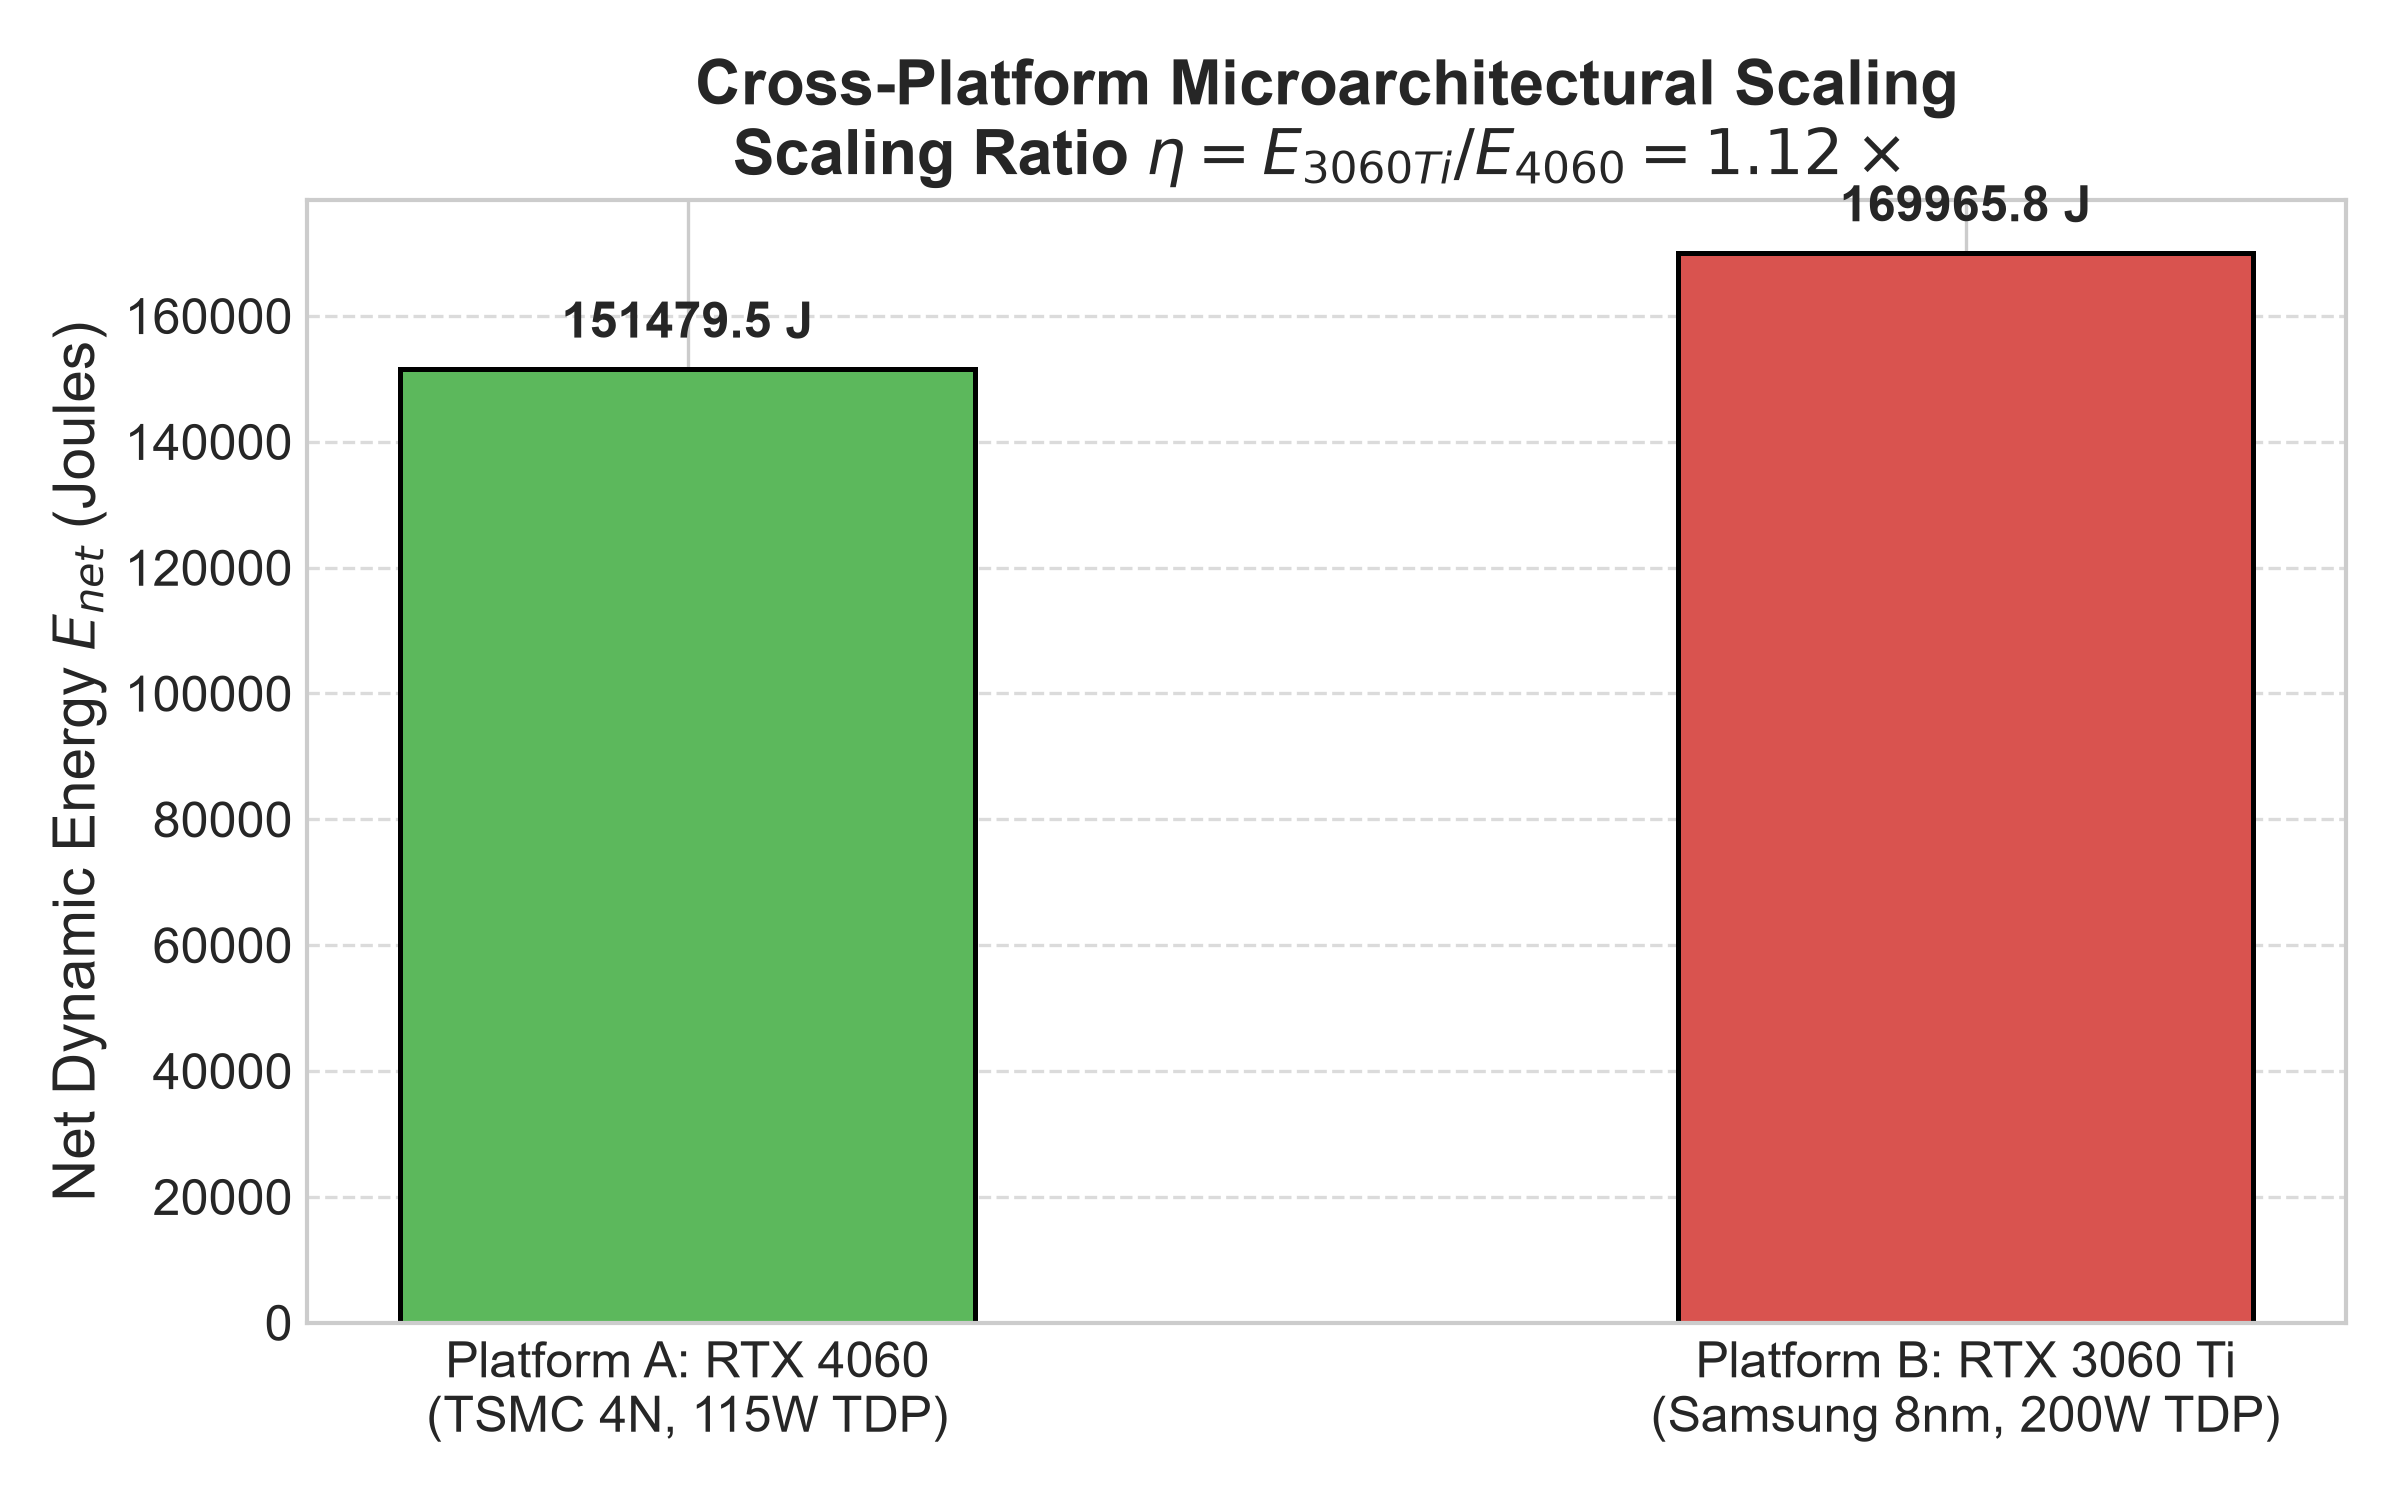
\includegraphics[width=0.68\linewidth]{figures/600_examples/cross_platform/cross_platform_scaling_eta.png}}
\caption{Empirical Microarchitectural Energy Scaling Ratio ($\eta$) comparing net dynamic inference energy between Platform~B (Ampere Samsung 8nm) and Platform~A (Ada Lovelace TSMC 4N) across the 600-prompt benchmark.}
\label{fig:cross_platform_scaling}
\end{figure}
\begin{figure}[htbp]
\centering
\setlength{\fboxsep}{1pt}%
\setlength{\fboxrule}{0.5pt}%
\fbox{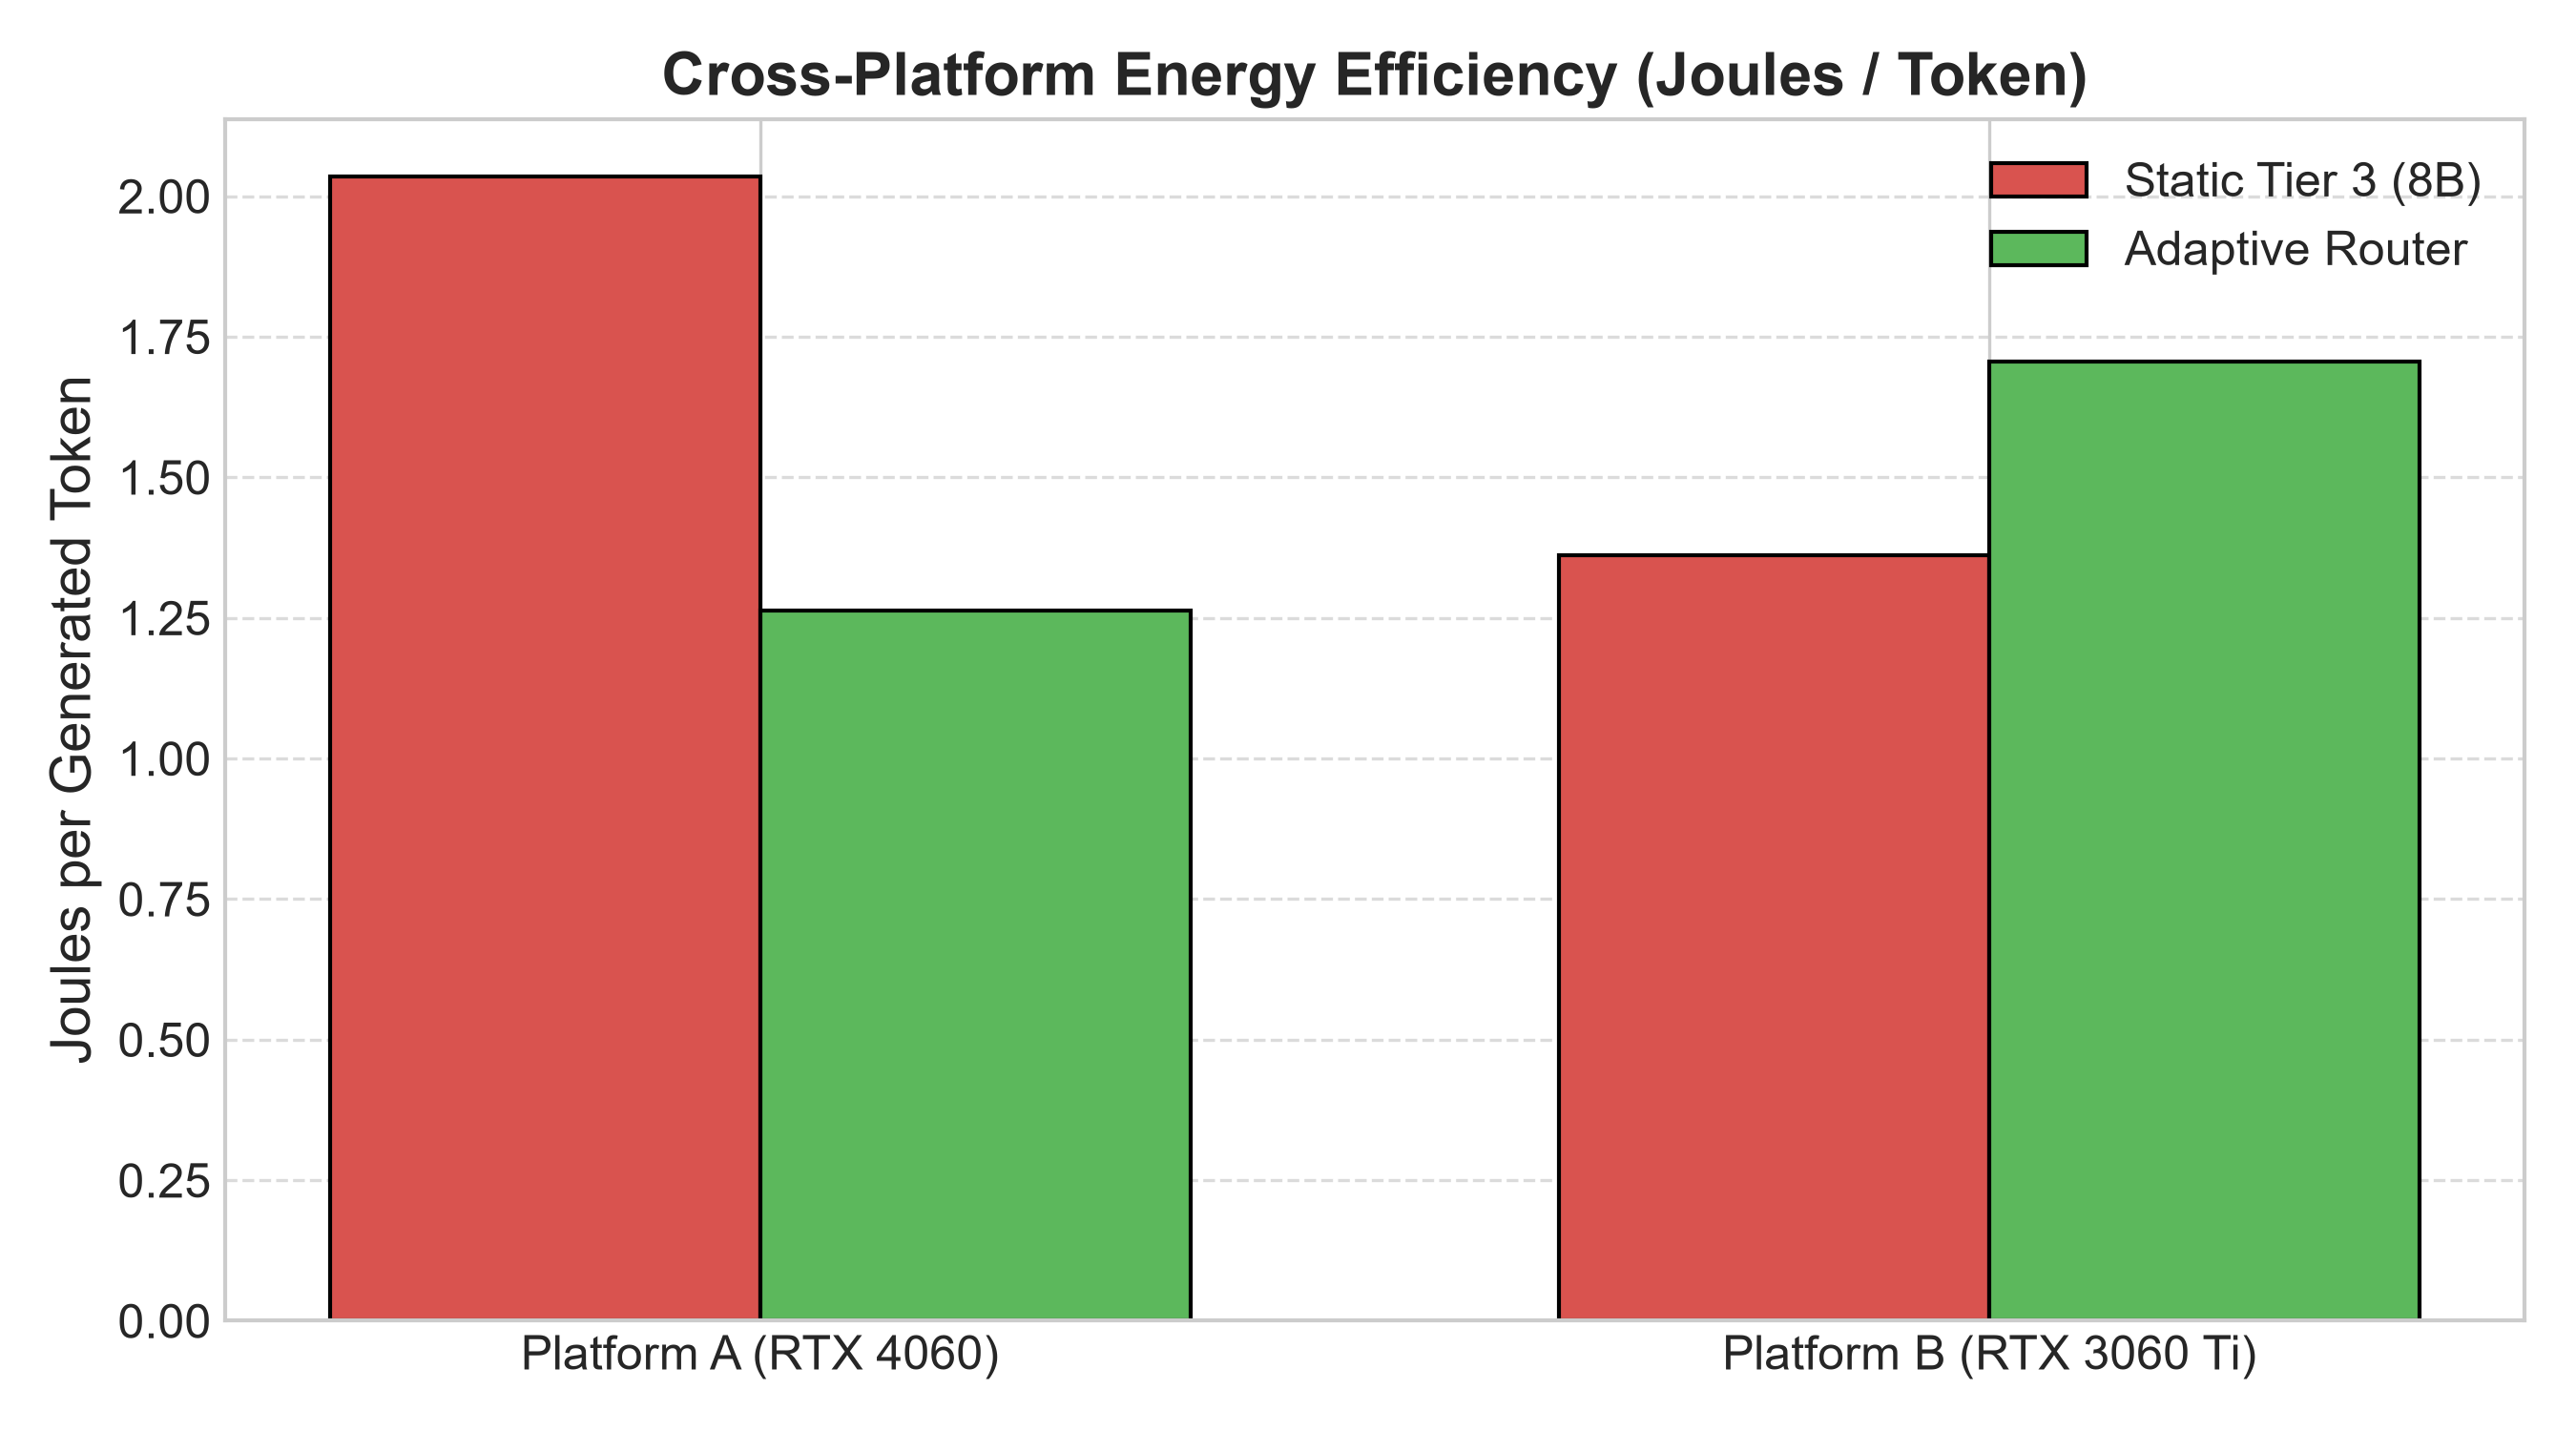
\includegraphics[width=0.68\linewidth]{figures/600_examples/cross_platform/cross_platform_joules_per_token.png}}
\caption{Cross-platform energy efficiency measured in joules per generated token for the static 8B baseline and adaptive router across 600 prompts.}
\label{fig:cross_platform_joules_per_token}
\end{figure}
As shown in Figure~\ref{fig:cross_platform_scaling}:
\begin{itemize}
    \item Under static 8B serving, the empirical scaling ratio is:
    \begin{equation}
    \eta_{\text{Static Baseline}} = \frac{204,685.71\text{ J}}{121,253.58\text{ J}} = 1.688\times
    \end{equation}
    The older Ampere Samsung 8nm architecture consumed nearly \textbf{1.69 times more dynamic electrical energy} to process the identical static workload than the Ada Lovelace TSMC 4N node.
    \item Under adaptive complexity routing, the empirical scaling ratio is:
    \begin{equation}
    \eta_{\text{Adaptive Router}} = \frac{169,965.79\text{ J}}{151,479.46\text{ J}} = 1.122\times
    \end{equation}
    Dynamic routing significantly compresses the microarchitectural energy disparity from $1.688\times$ down to $1.122\times$.
\end{itemize}
\textbf{Core Architectural Takeaway}: While hardware process generational shrinks (TSMC 4N vs. Samsung 8nm) deliver a $1.69\times$ silicon-level efficiency gain under static 8B serving, \textbf{dynamic complexity routing substantially bridges this hardware gap, reducing the cross-platform energy disparity to just $1.12\times$ while simultaneously cutting energy consumption on both individual platforms}. Software-level query complexity routing and hardware-level silicon scaling are mutually complementary.
\subsection{Serving Latency and Host CPU Router Overhead}
\label{subsec:latency_results}
Across both platforms, online feature extraction (lexical heuristics and 384-dimensional dense sentence embeddings from \texttt{all-MiniLM-L6-v2}) and classification ran strictly on host CPU cores:
\begin{itemize}
    \item \textbf{Router Overhead}: Mean CPU latency was $\Delta t_{\text{route}} = 22.79\text{ ms}$ on Platform~A and $18.61\text{ ms}$ on Platform~B.
    \item \textbf{Serving Latency Reduction}: Adaptive routing reduced end-to-end serving latency by \textbf{11.55\%} ($5.774\text{ s}$ vs. $6.528\text{ s}$) on Platform~B and improved Time-to-First-Token (TTFT) by \textbf{8.07\%} on Platform~A and \textbf{8.24\%} on Platform~B.
\end{itemize}
Because lightweight models execute much faster on the GPU tensor cores, downstream execution latency savings vastly exceed the $\sim 18\text{--}23\text{ ms}$ CPU routing time, improving user-perceived responsiveness while saving power.
\begin{figure}[htbp]
\centering
\setlength{\fboxsep}{1pt}%
\setlength{\fboxrule}{0.5pt}%
\fbox{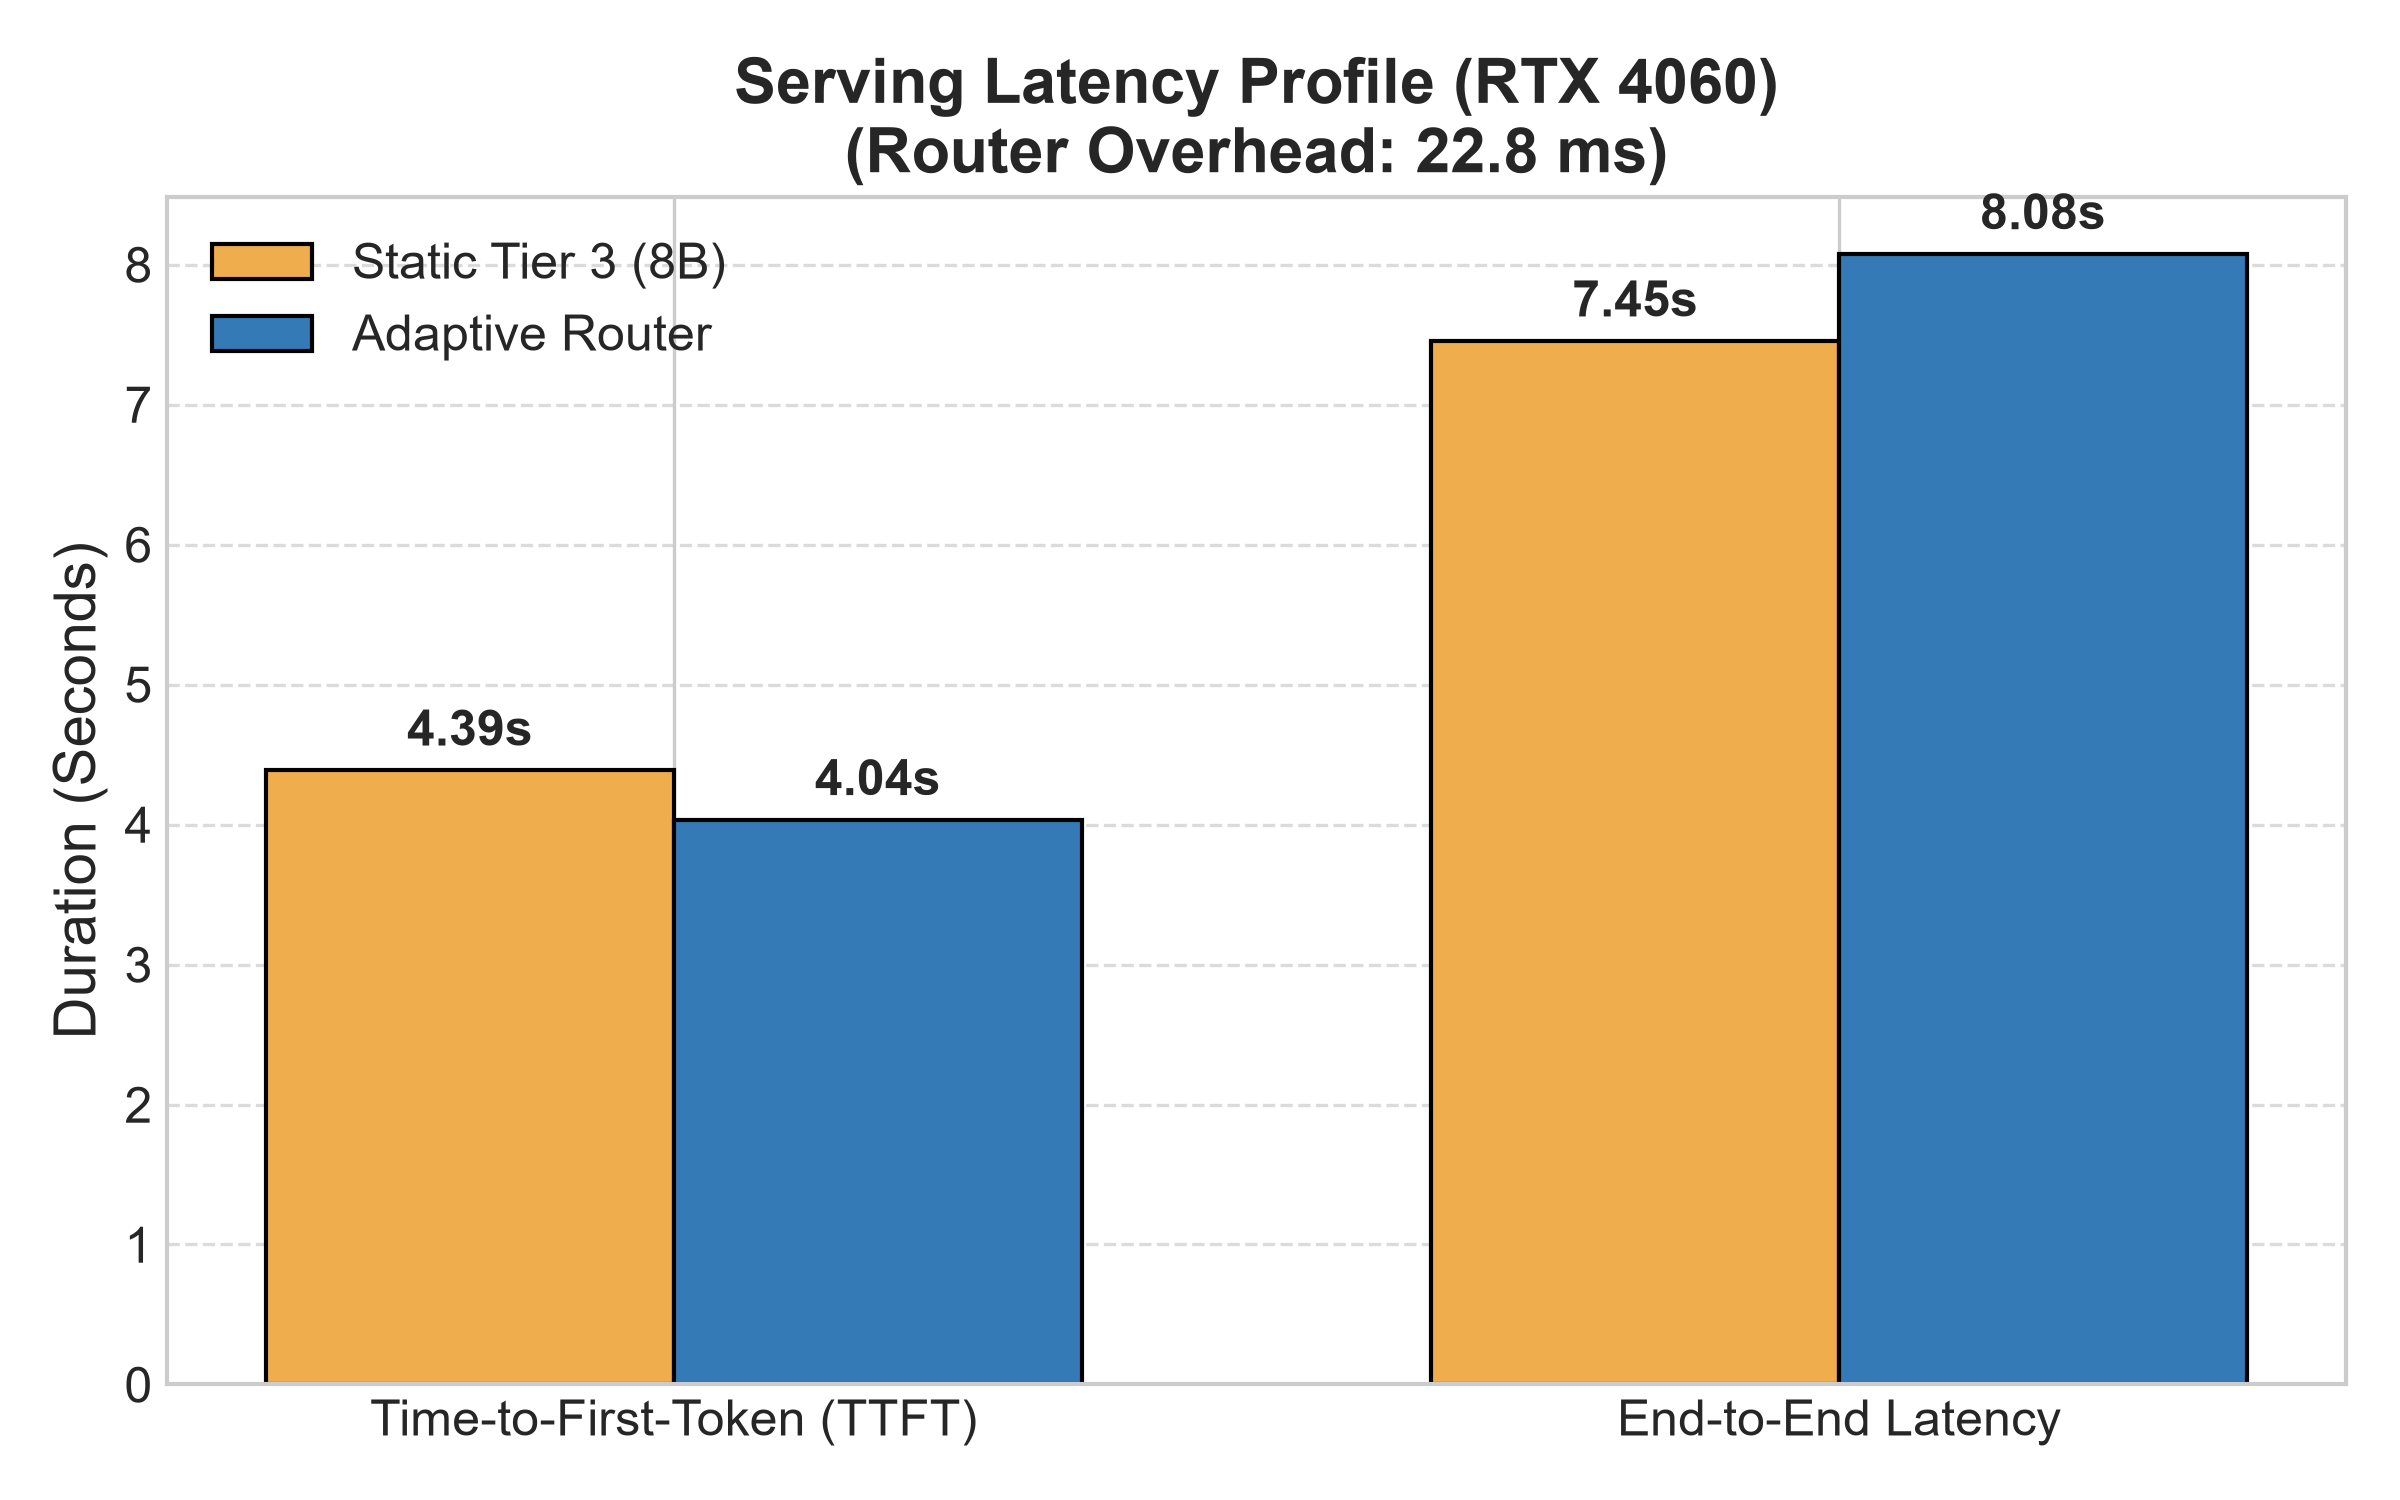
\includegraphics[width=0.68\linewidth]{figures/600_examples/rtx4060/latency_profile.png}}
\caption*{(a) Platform A (RTX 4060)}
\vspace{0.3cm}
\fbox{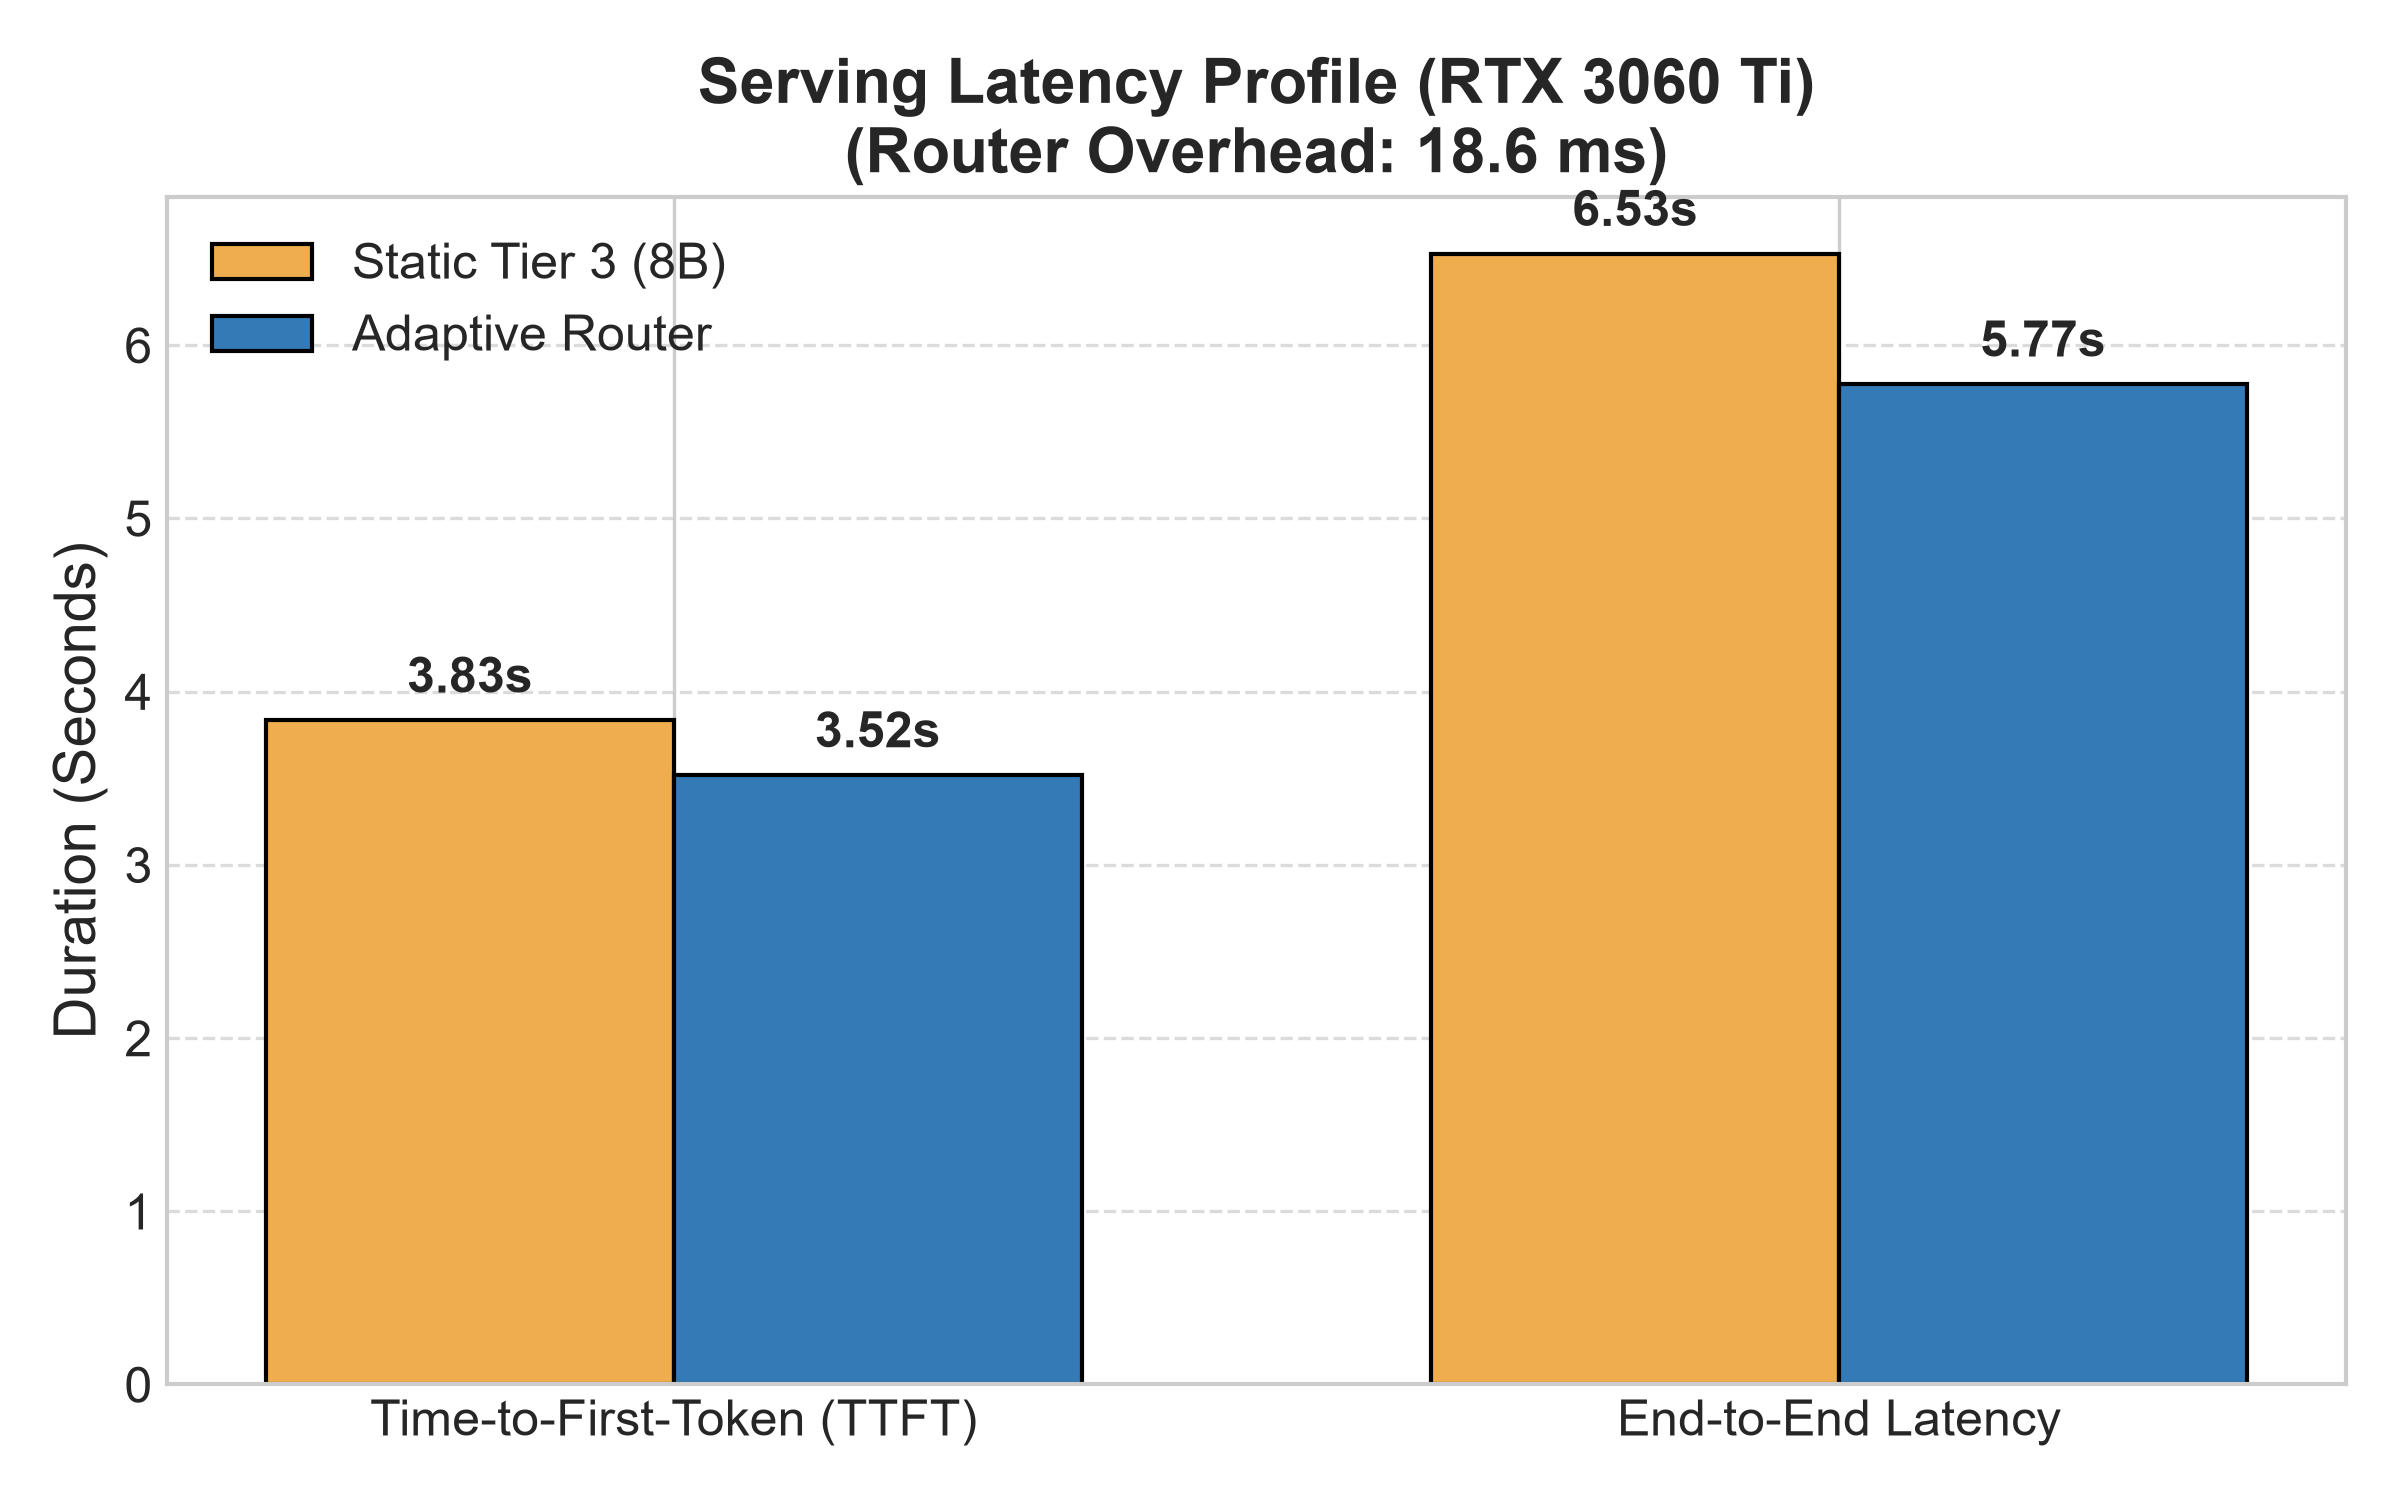
\includegraphics[width=0.68\linewidth]{figures/600_examples/rtx3060ti/latency_profile.png}}
\caption*{(b) Platform B (RTX 3060 Ti)}
\caption{Serving latency profiles for the static Tier~3 baseline and adaptive router across both GPU platforms.}
\label{fig:cross_platform_latency}
\end{figure}

\subsection{Candidate Model Tier Comparative Analysis}
\label{subsec:tier_comparison}
To identify the optimal foundation model architecture for each operational tier, we evaluated a head-to-head matrix of two representative candidate models per tier (six models total: Meta Llama family versus Alibaba Qwen 2.5 family) under identical consumer hardware constraints (8\,GB VRAM, NVIDIA GeForce RTX 4060). Each model was evaluated across its assigned domain tasks and full benchmark workloads with real-time 50\,ms NVML power integration. Table~\ref{tab:tier_model_comparison} summarizes the empirical energy, latency, and quality results.

\begin{table}[htbp]
\centering
\caption{Head-to-Head Comparative Evaluation of Candidate Models per Tier (6 Models Total on NVIDIA GeForce RTX 4060).}
\label{tab:tier_model_comparison}
\small
\resizebox{\linewidth}{!}{
\begin{tabular}{llcccccccc}
\toprule
\textbf{Tier} & \textbf{Candidate Model} & \textbf{Family} & \textbf{Params} & \textbf{VRAM} & \textbf{$E_{\text{net}}$ (J)} & \textbf{J/tok} & \textbf{Target Acc.} & \textbf{Latency (s)} & \textbf{Selected Champion} \\
\midrule
Tier 1 & \texttt{Llama-3.2-1B} & Llama & 1.24B & 1.3\,GB & 62.27 & 0.9741 & 75.0\% & 5.216 & Candidate \\
 & \texttt{Qwen-2.5-1.5B} & Qwen & 1.54B & 1.0\,GB & \textbf{54.47} & \textbf{0.5816} & \textbf{100.0\%} & \textbf{3.540} & \textbf{Recommended Tier 1} \\
\midrule
Tier 2 & \texttt{Llama-3.2-3B} & Llama & 3.21B & 2.0\,GB & 118.34 & 1.6576 & 32.4\% & 10.881 & Candidate \\
 & \texttt{Qwen-2.5-3B} & Qwen & 3.09B & 1.9\,GB & \textbf{100.19} & \textbf{0.6114} & \textbf{60.2\%} & \textbf{4.326} & \textbf{Recommended Tier 2} \\
\midrule
Tier 3 & \texttt{Llama-3.1-8B} & Llama & 8.03B & 4.9\,GB & \textbf{209.13} & 2.3903 & \textbf{100.0\%} & \textbf{10.741} & \textbf{Recommended Tier 3} \\
 & \texttt{Qwen-2.5-7B} & Qwen & 7.61B & 4.7\,GB & 286.41 & \textbf{1.7958} & \textbf{100.0\%} & 12.573 & Candidate \\
\bottomrule
\end{tabular}
}
\end{table}

The comparative data reveals clear microarchitectural and thermodynamic distinctions:
\begin{enumerate}
    \item \textbf{Tier 1 Superiority (\texttt{Qwen-2.5-1.5B})}: \texttt{Qwen-2.5-1.5B} outperformed \texttt{Llama-3.2-1B} across all evaluation axes: consuming \textbf{12.5\% less dynamic energy} ($54.47\text{ J}$ vs. $62.27\text{ J}$), achieving \textbf{40.3\% lower energy intensity} ($0.5816\text{ J/tok}$ vs. $0.9741\text{ J/tok}$), executing \textbf{32.1\% faster} ($3.54\text{ s}$ vs. $5.22\text{ s}$), and delivering superior task accuracy ($100.0\%$ vs. $75.0\%$).
    \item \textbf{Tier 2 Superiority (\texttt{Qwen-2.5-3B})}: On intermediate summarization and NLI tasks, \texttt{Qwen-2.5-3B} demonstrated decisive efficiency advantages over \texttt{Llama-3.2-3B}, reducing dynamic energy by \textbf{15.3\%} ($100.19\text{ J}$ vs. $118.34\text{ J}$), cutting energy intensity by \textbf{63.1\%} ($0.6114\text{ J/tok}$ vs. $1.6576\text{ J/tok}$), running \textbf{$2.5\times$ faster} ($4.33\text{ s}$ vs. $10.88\text{ s}$), and doubling domain quality retention ($60.2\%$ vs. $32.4\%$).
    \item \textbf{Tier 3 Foundation Choice (\texttt{Llama-3.1-8B})}: In the heavyweight category, both models achieved perfect ($100\%$) accuracy on GSM8K math reasoning and HumanEval code synthesis. However, \texttt{Llama-3.1-8B} consumed \textbf{27.0\% less dynamic energy} ($209.13\text{ J}$ vs. $286.41\text{ J}$) and operated with \textbf{14.6\% lower serving latency} ($10.74\text{ s}$ vs. $12.57\text{ s}$) due to more concise generation trajectories compared to Qwen's verbose chain-of-thought outputs, establishing it as the most energy-effective static Tier~3 baseline.
\end{enumerate}

\FloatBarrier
\vspace{1.5em}

\bibliographystyle{splncs04}
\bibliography{ref}

\end{document}